\section{Single-Agent Experiment: CartSafe} 
\label{appsec:cartsafe_results}

 
\begin{figure*}[h!]
    \centering
    \begin{minipage}[b]{0.32\textwidth}
        \centering
        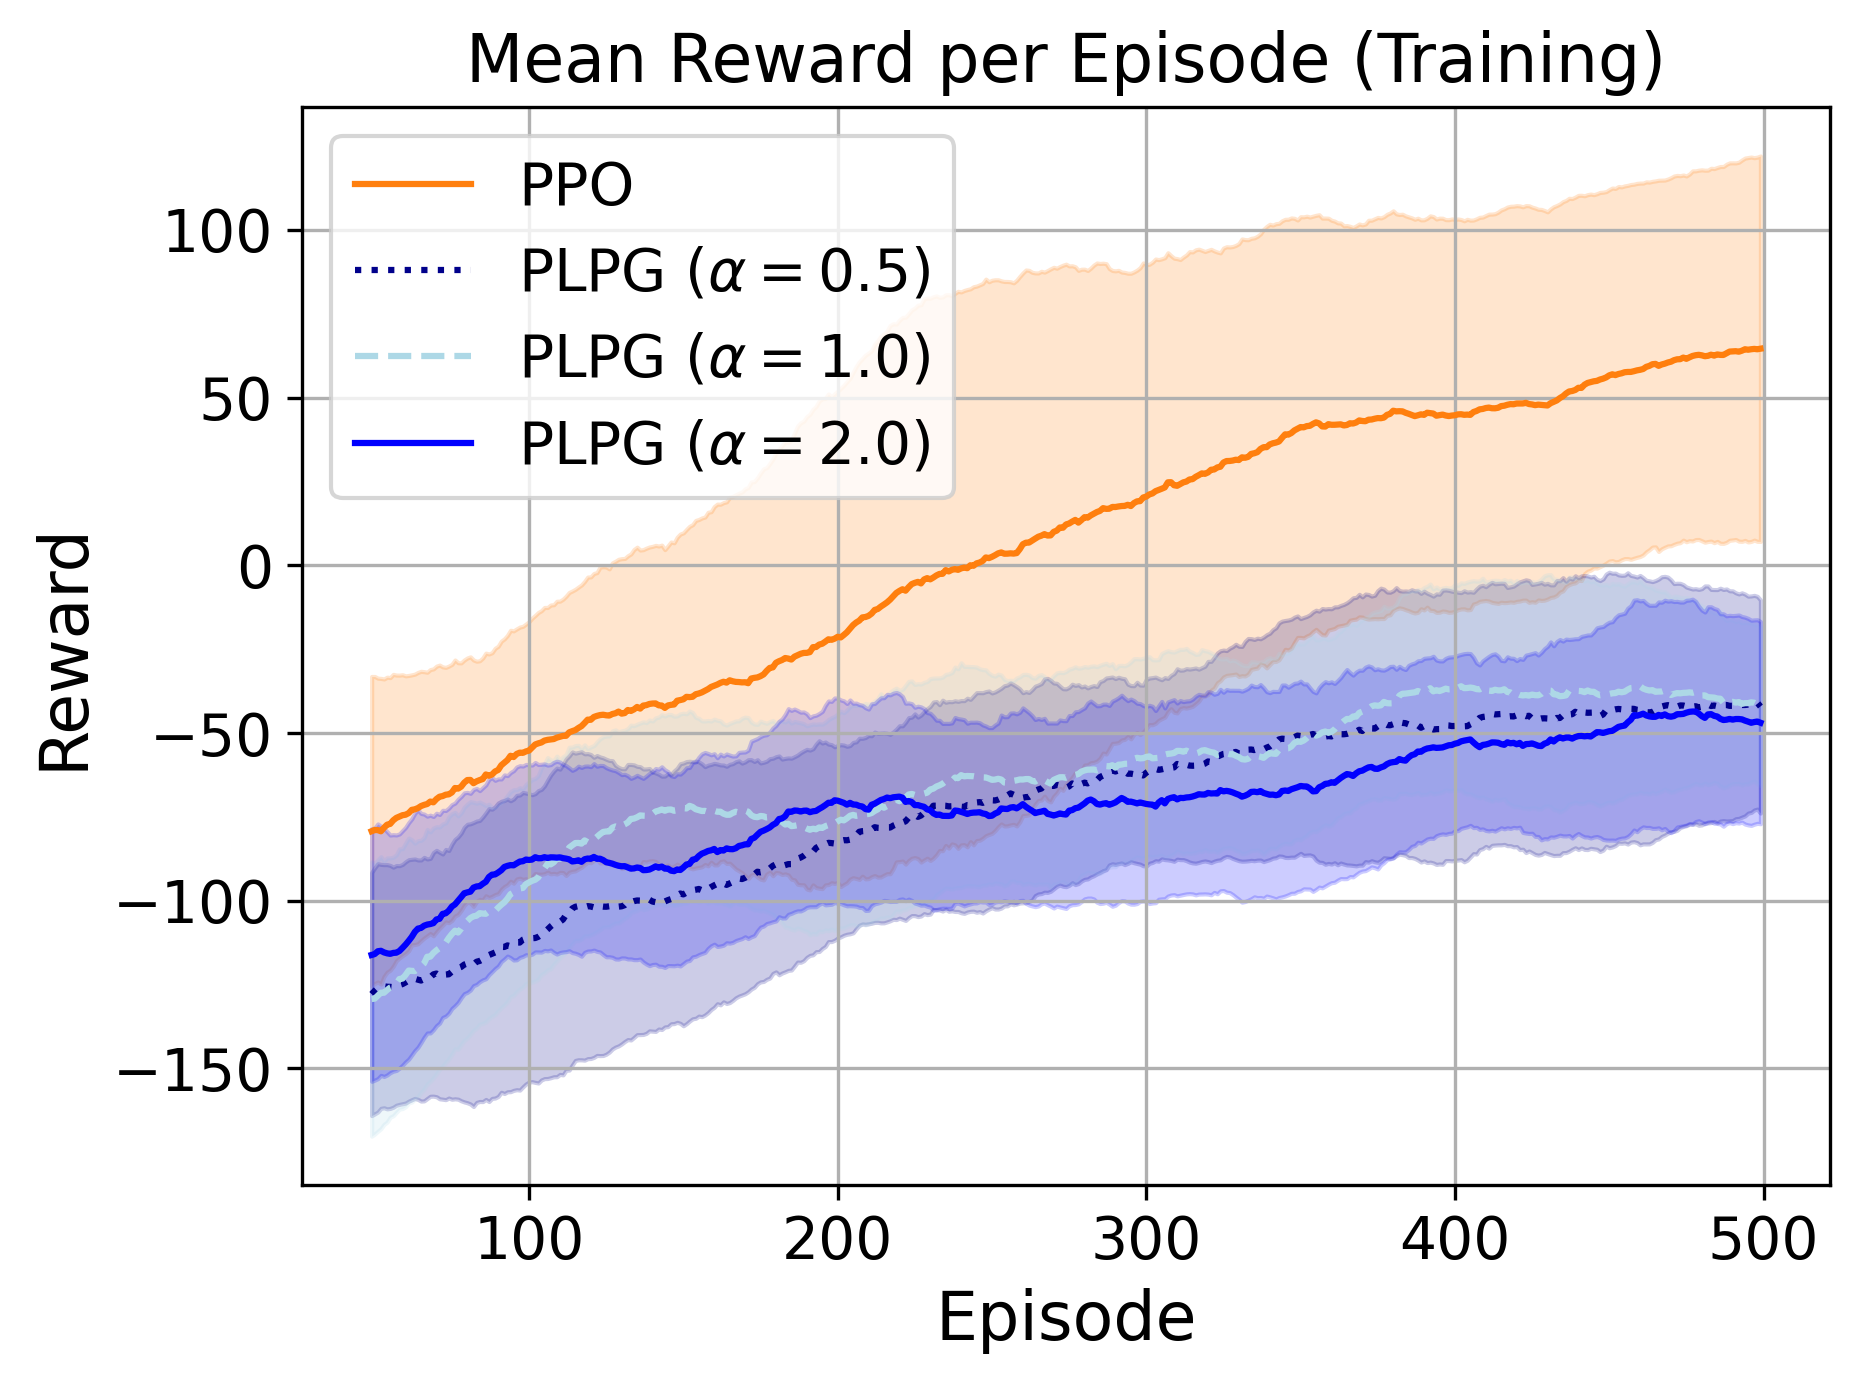
\includegraphics[width=\textwidth]{Experiments/images/cartsafe/training_CartSafe-v0_ppo.png}
        \vspace{0.3em}

        \textbf{(a)}
        \label{fig:subfig1}
    \end{minipage}
    \hfill
    \begin{minipage}[b]{0.32\textwidth}
        \centering
        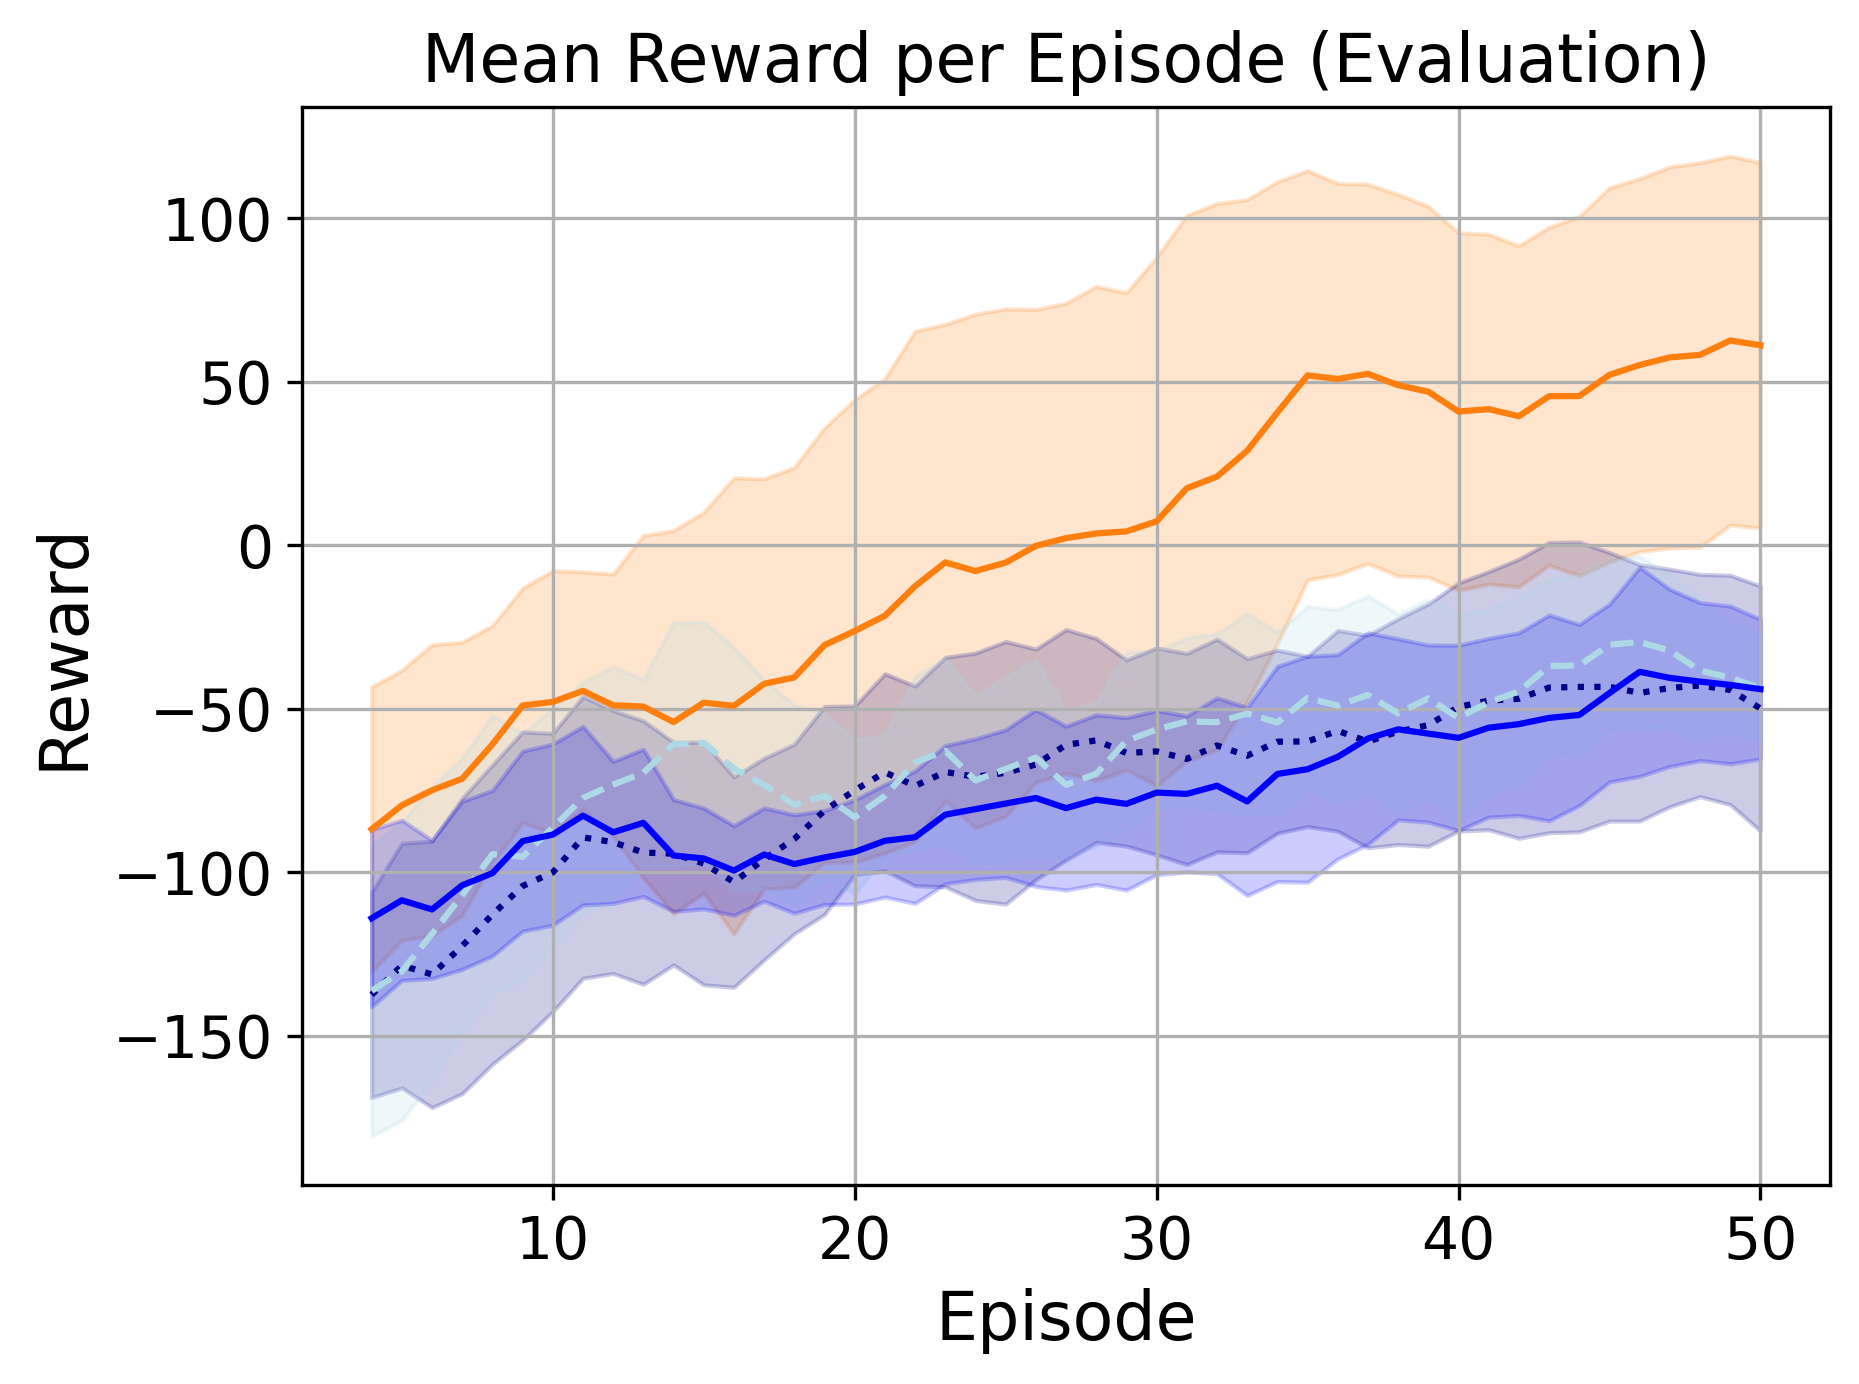
\includegraphics[width=\textwidth]{Experiments/images/cartsafe/eval_CartSafe-v0_ppo.png}
        \vspace{0.3em}

        \textbf{(b)}
        \label{fig:subfig2}
    \end{minipage}
    \hfill
    \begin{minipage}[b]{0.32\textwidth}
        \centering
        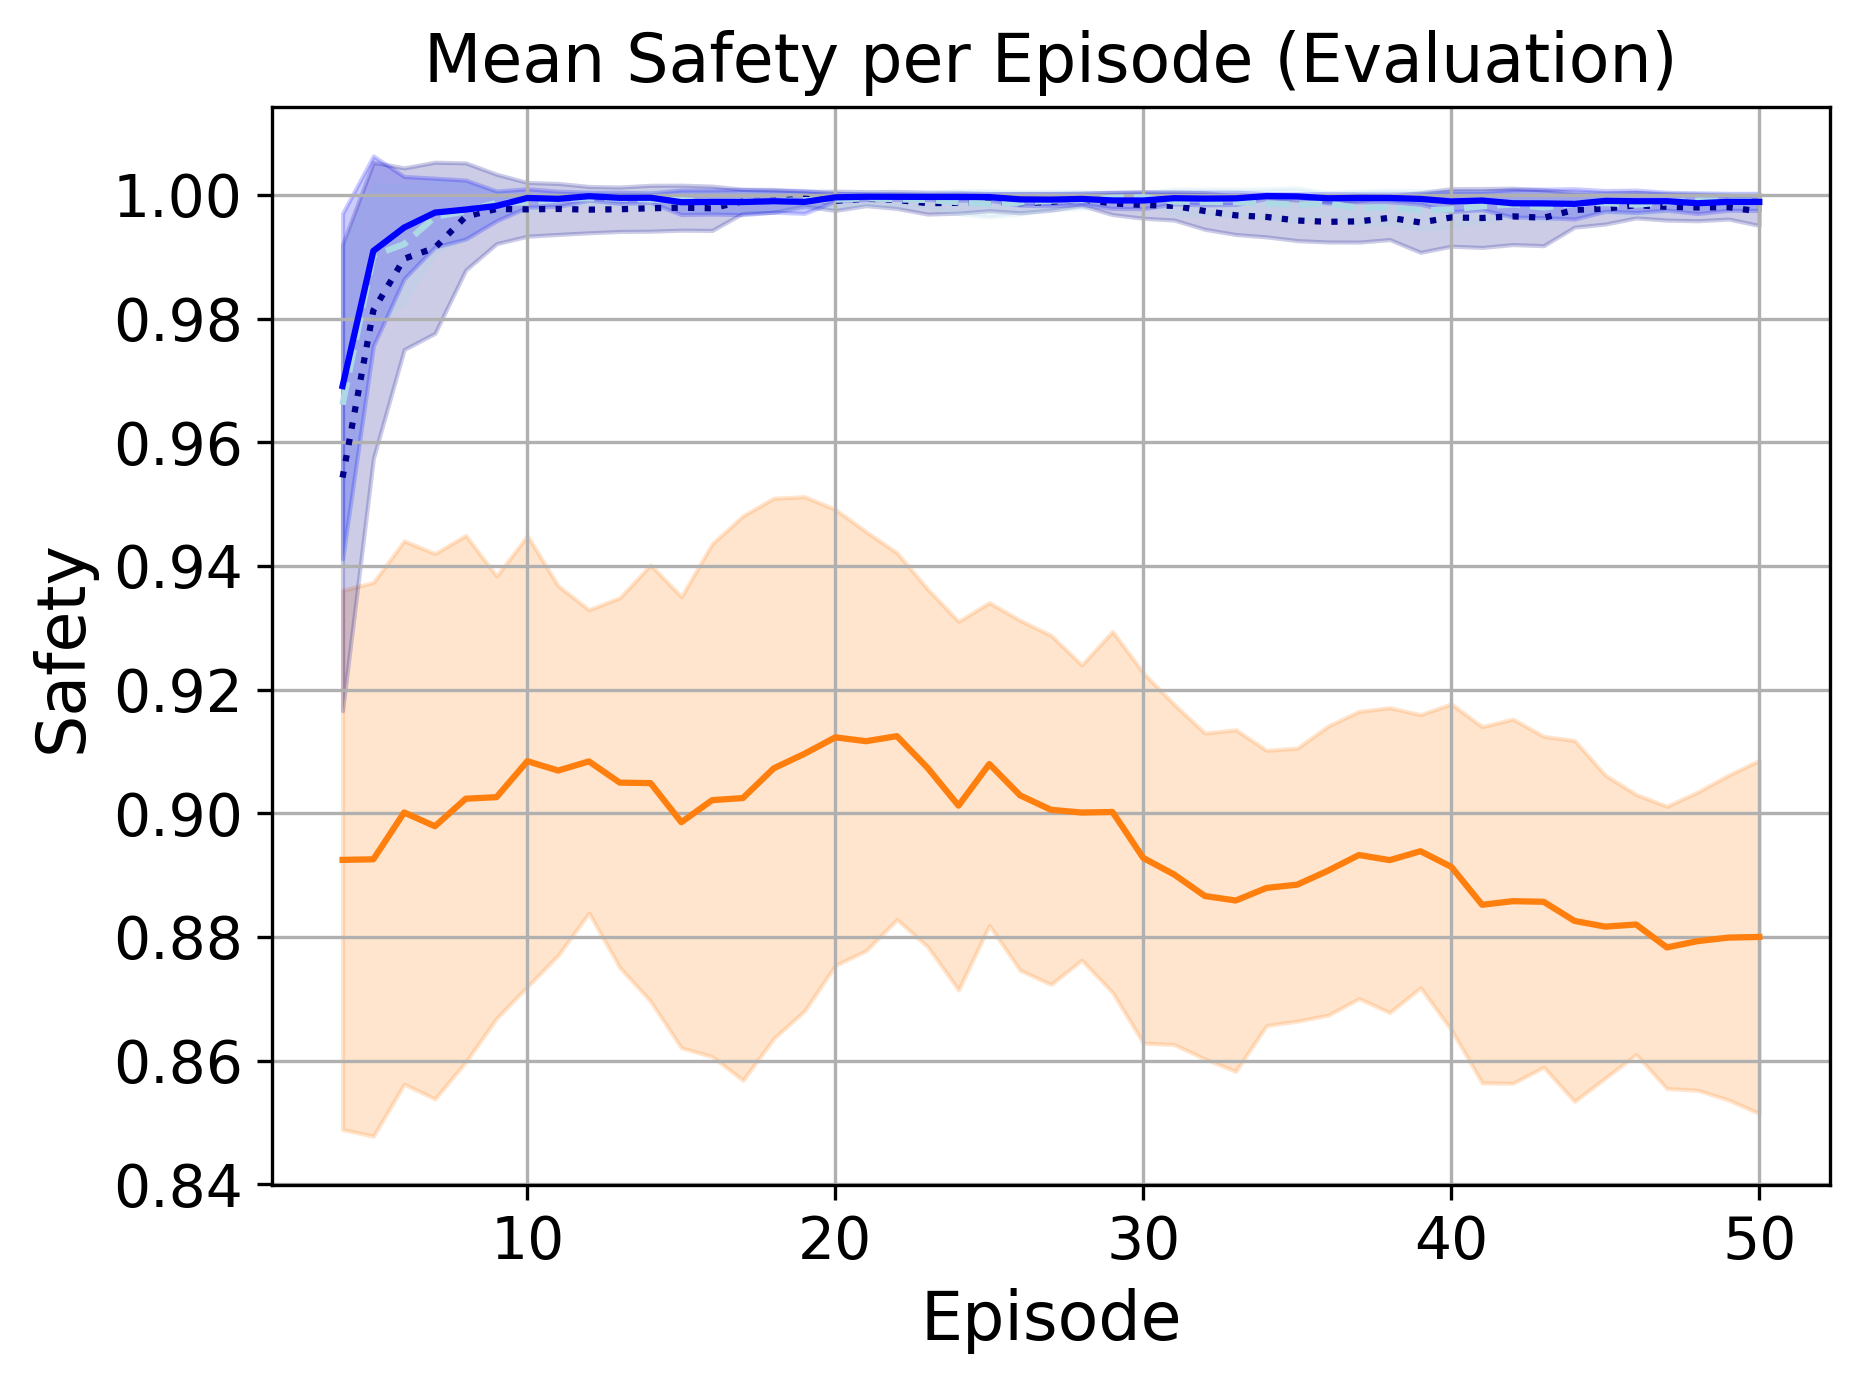
\includegraphics[width=\textwidth]{Experiments/images/cartsafe/safety_CartSafe-v0_ppo.png}
        \vspace{0.3em}

        \textbf{(c)}
        \label{fig:subfig3}
    \end{minipage}

    \caption[Single-agent Results for \textit{CartSafe} (PLPG agents).]{Training, evaluation and safety results for \textit{CartSafe} for PPO-based agents. The lines represent the mean and the shadow the standard deviation over 5 seeds. Results are smoothed using a rolling average with window size 50.}
    \label{fig:cartsafe_ppo}
\end{figure*}
\begin{figure*}[h!]
    \centering

    % First row: Off-policy, epsilon-greedy
    \begin{minipage}[b]{0.32\textwidth}
        \centering
        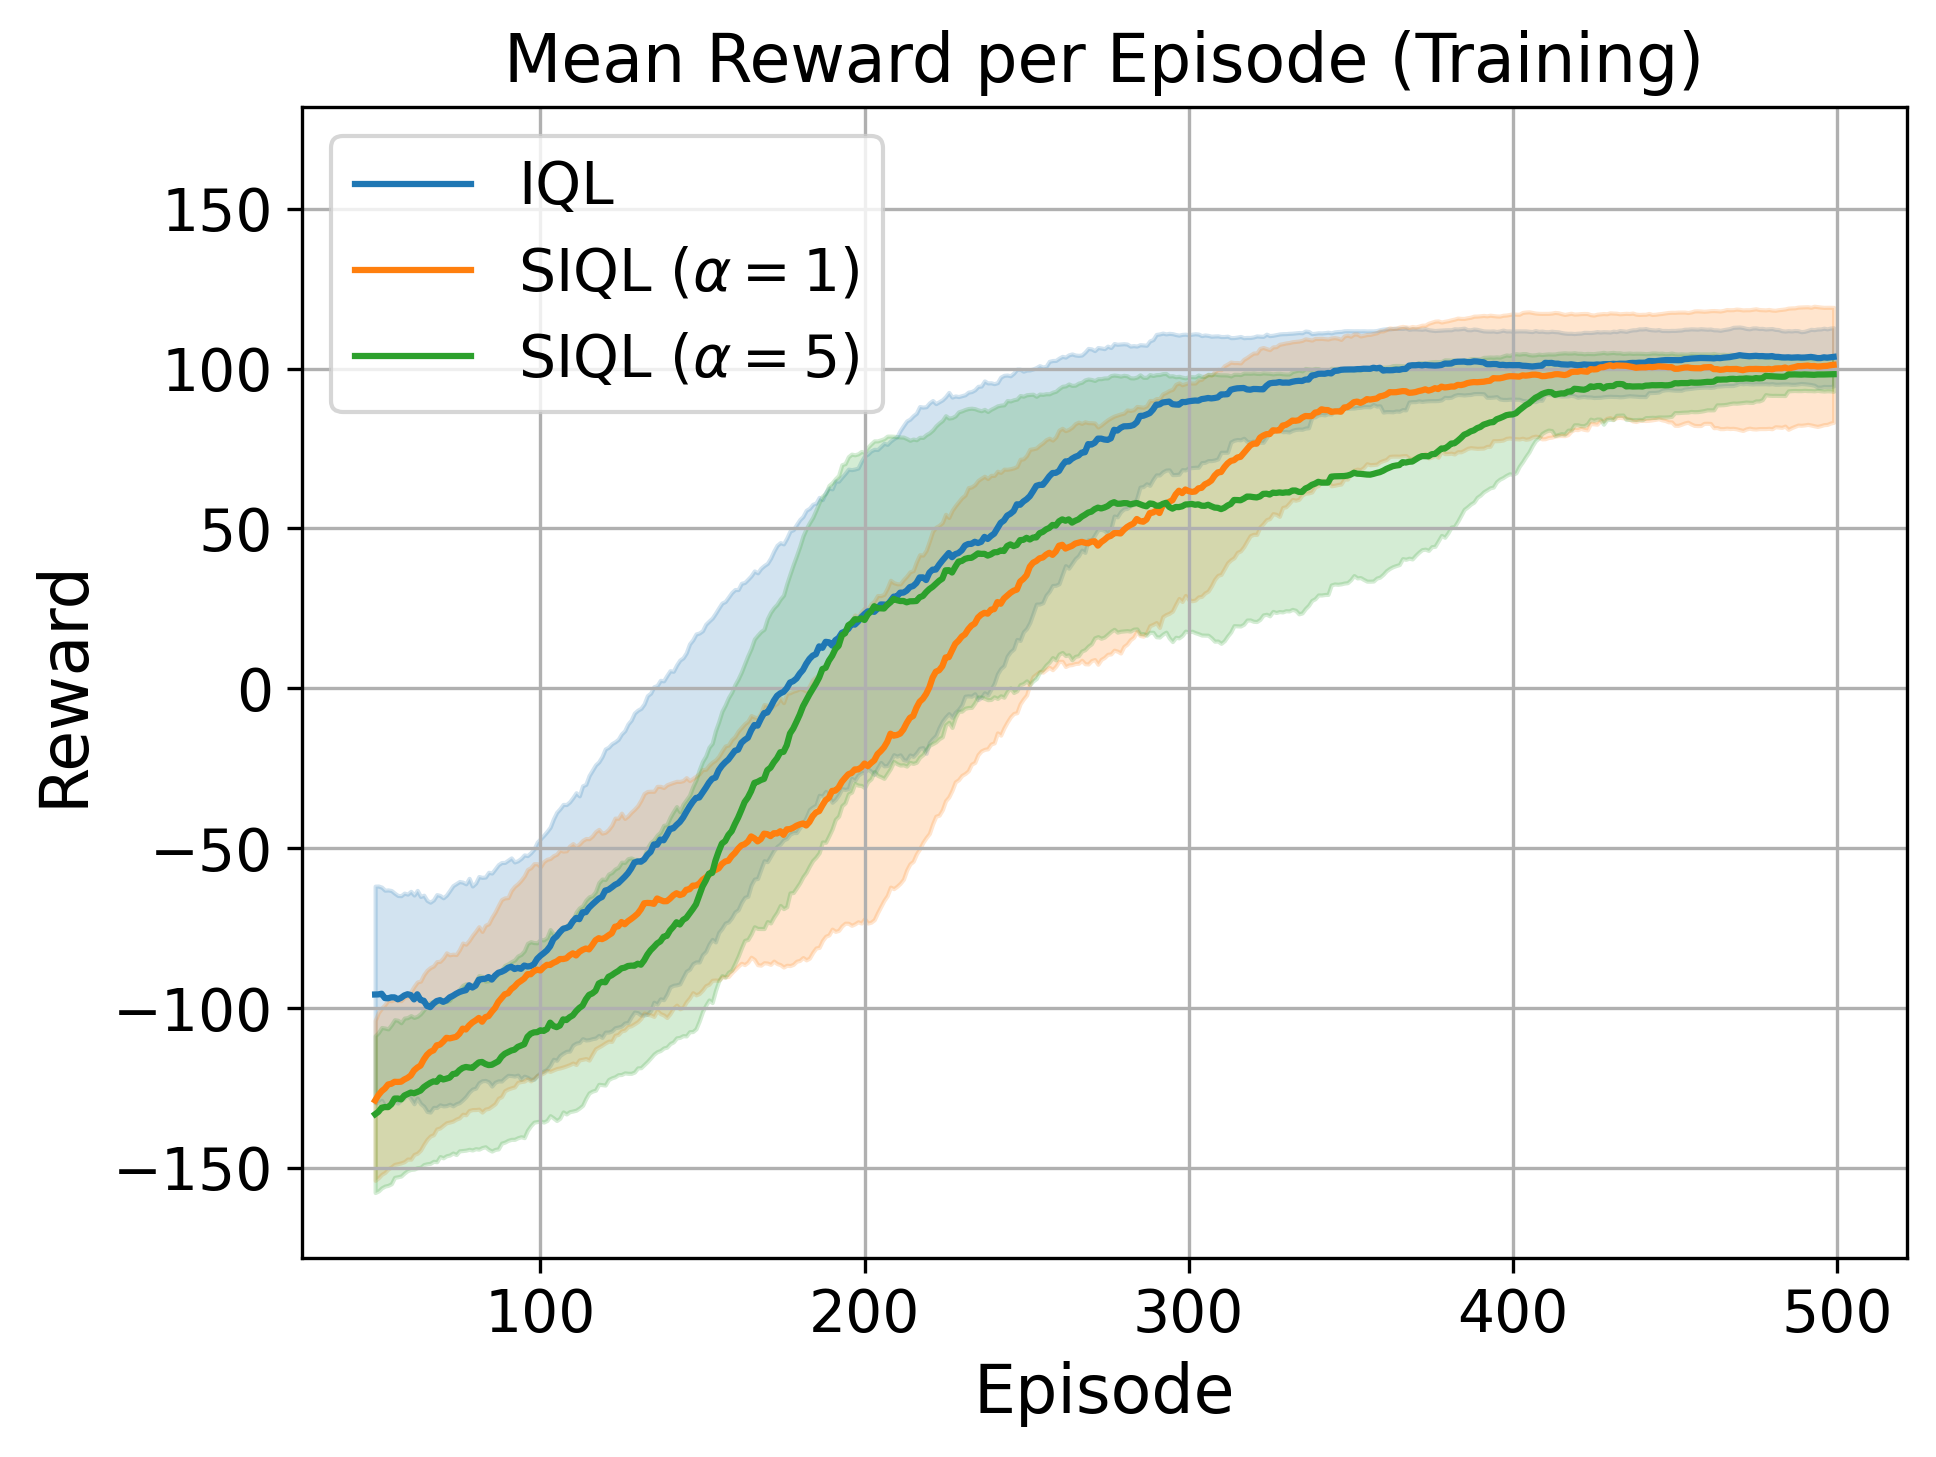
\includegraphics[width=\textwidth]{Experiments/images/cartsafe/training_DQN_greedy_cartsafe.png}
        \vspace{0.3em}

        \textbf{(a)}
        \label{fig:cartsafe_dqn:sub1}
    \end{minipage}
    \hfill
    \begin{minipage}[b]{0.32\textwidth}
        \centering
        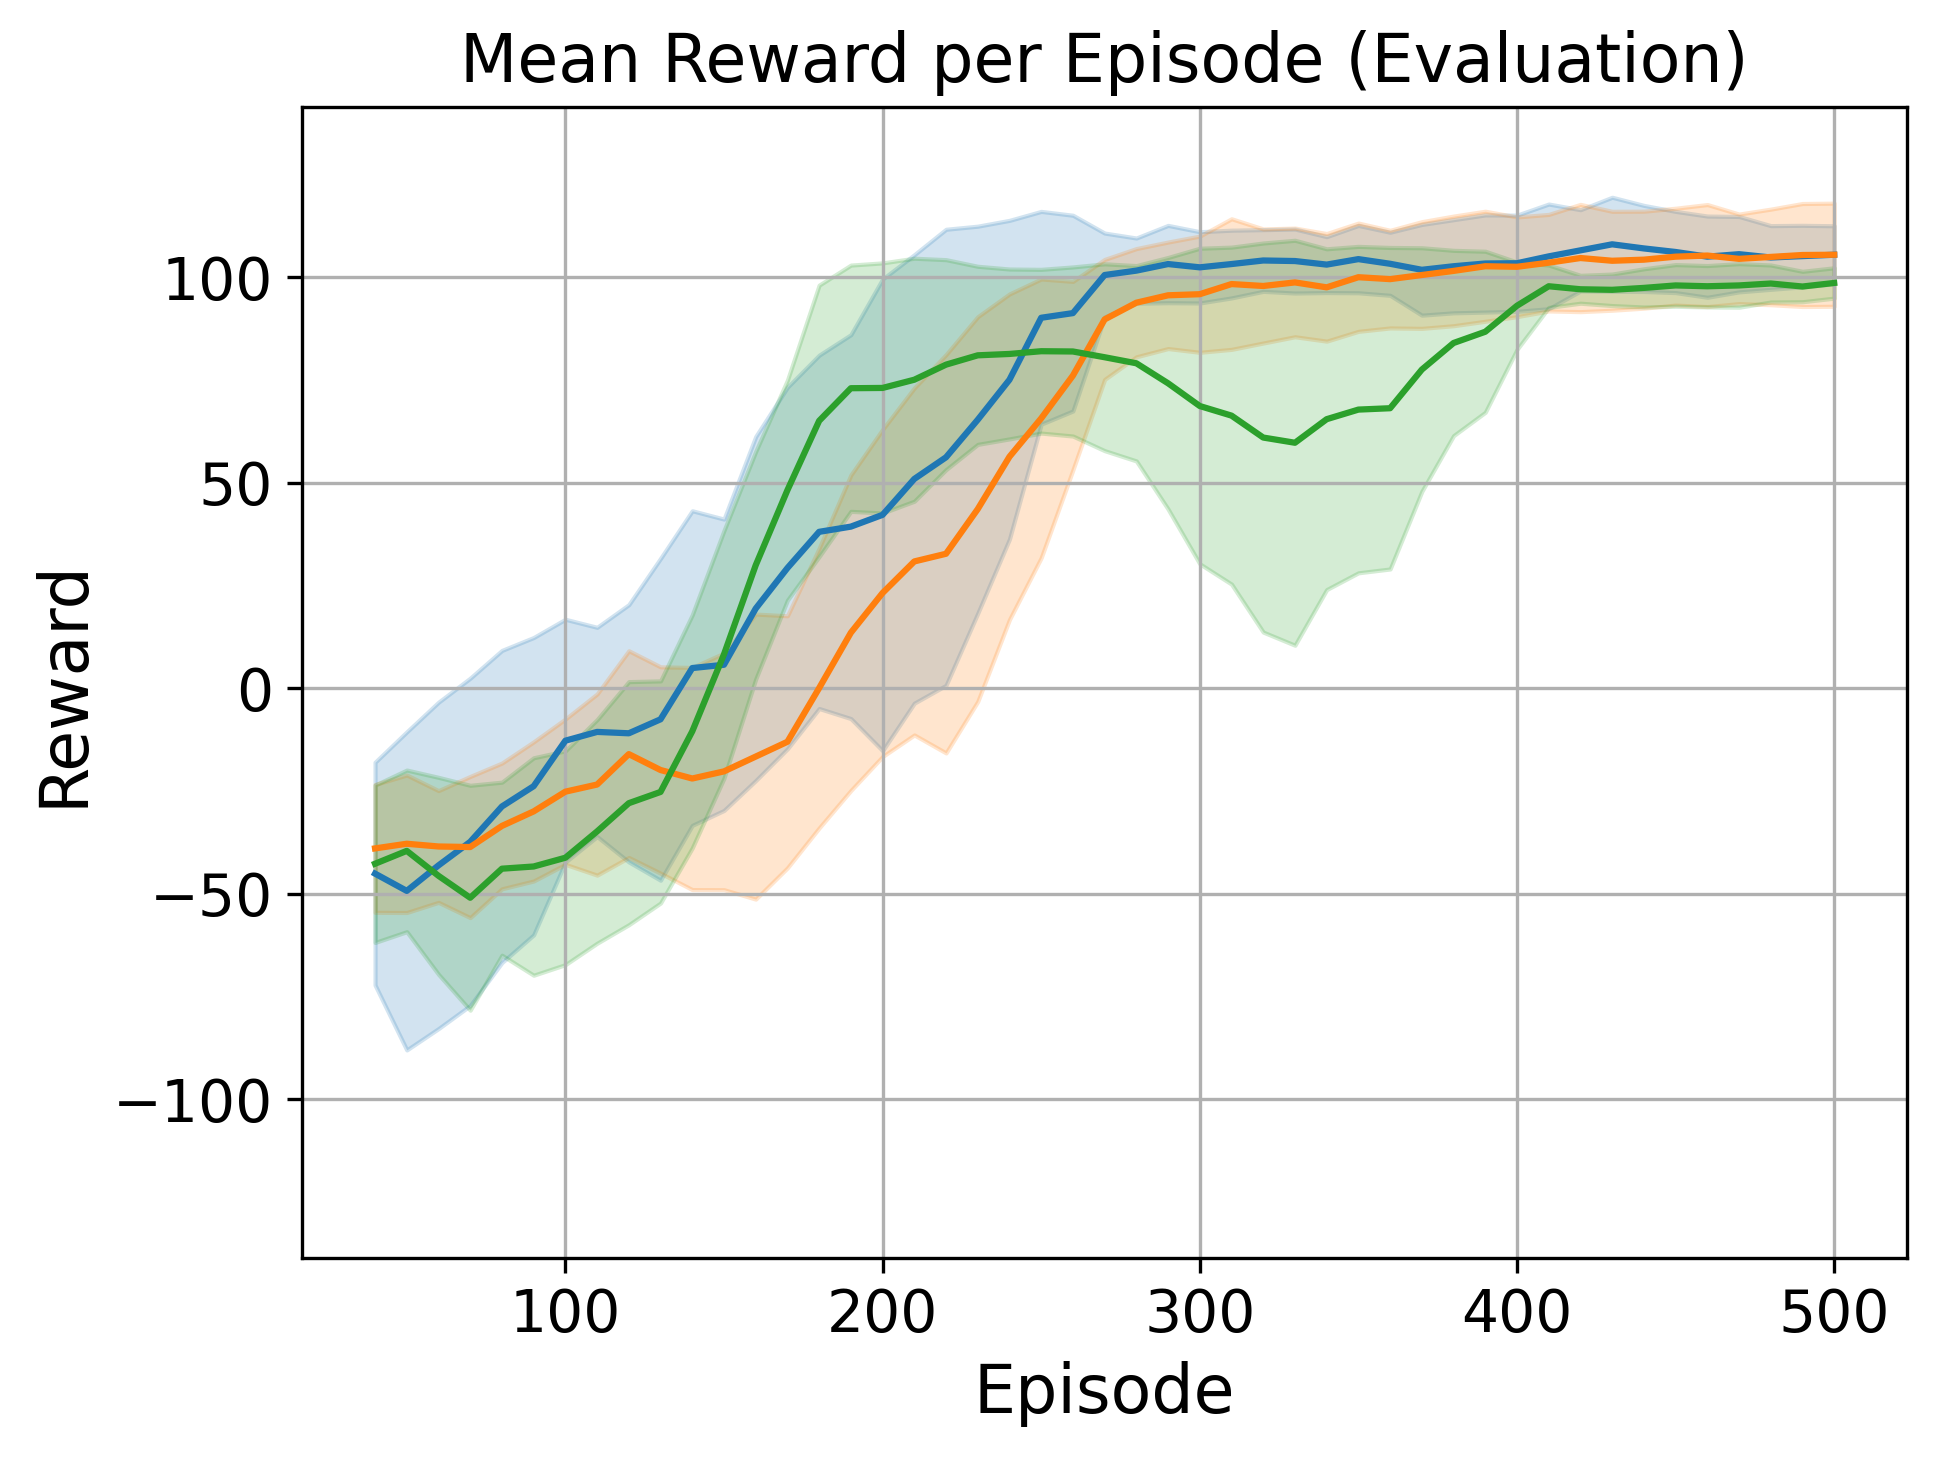
\includegraphics[width=\textwidth]{Experiments/images/cartsafe/eval_DQN_greedy_cartsafe.png}
        \vspace{0.3em}

        \textbf{(b)}
        \label{fig:cartsafe_dqn:sub2}
    \end{minipage}
    \hfill
    \begin{minipage}[b]{0.32\textwidth}
        \centering
        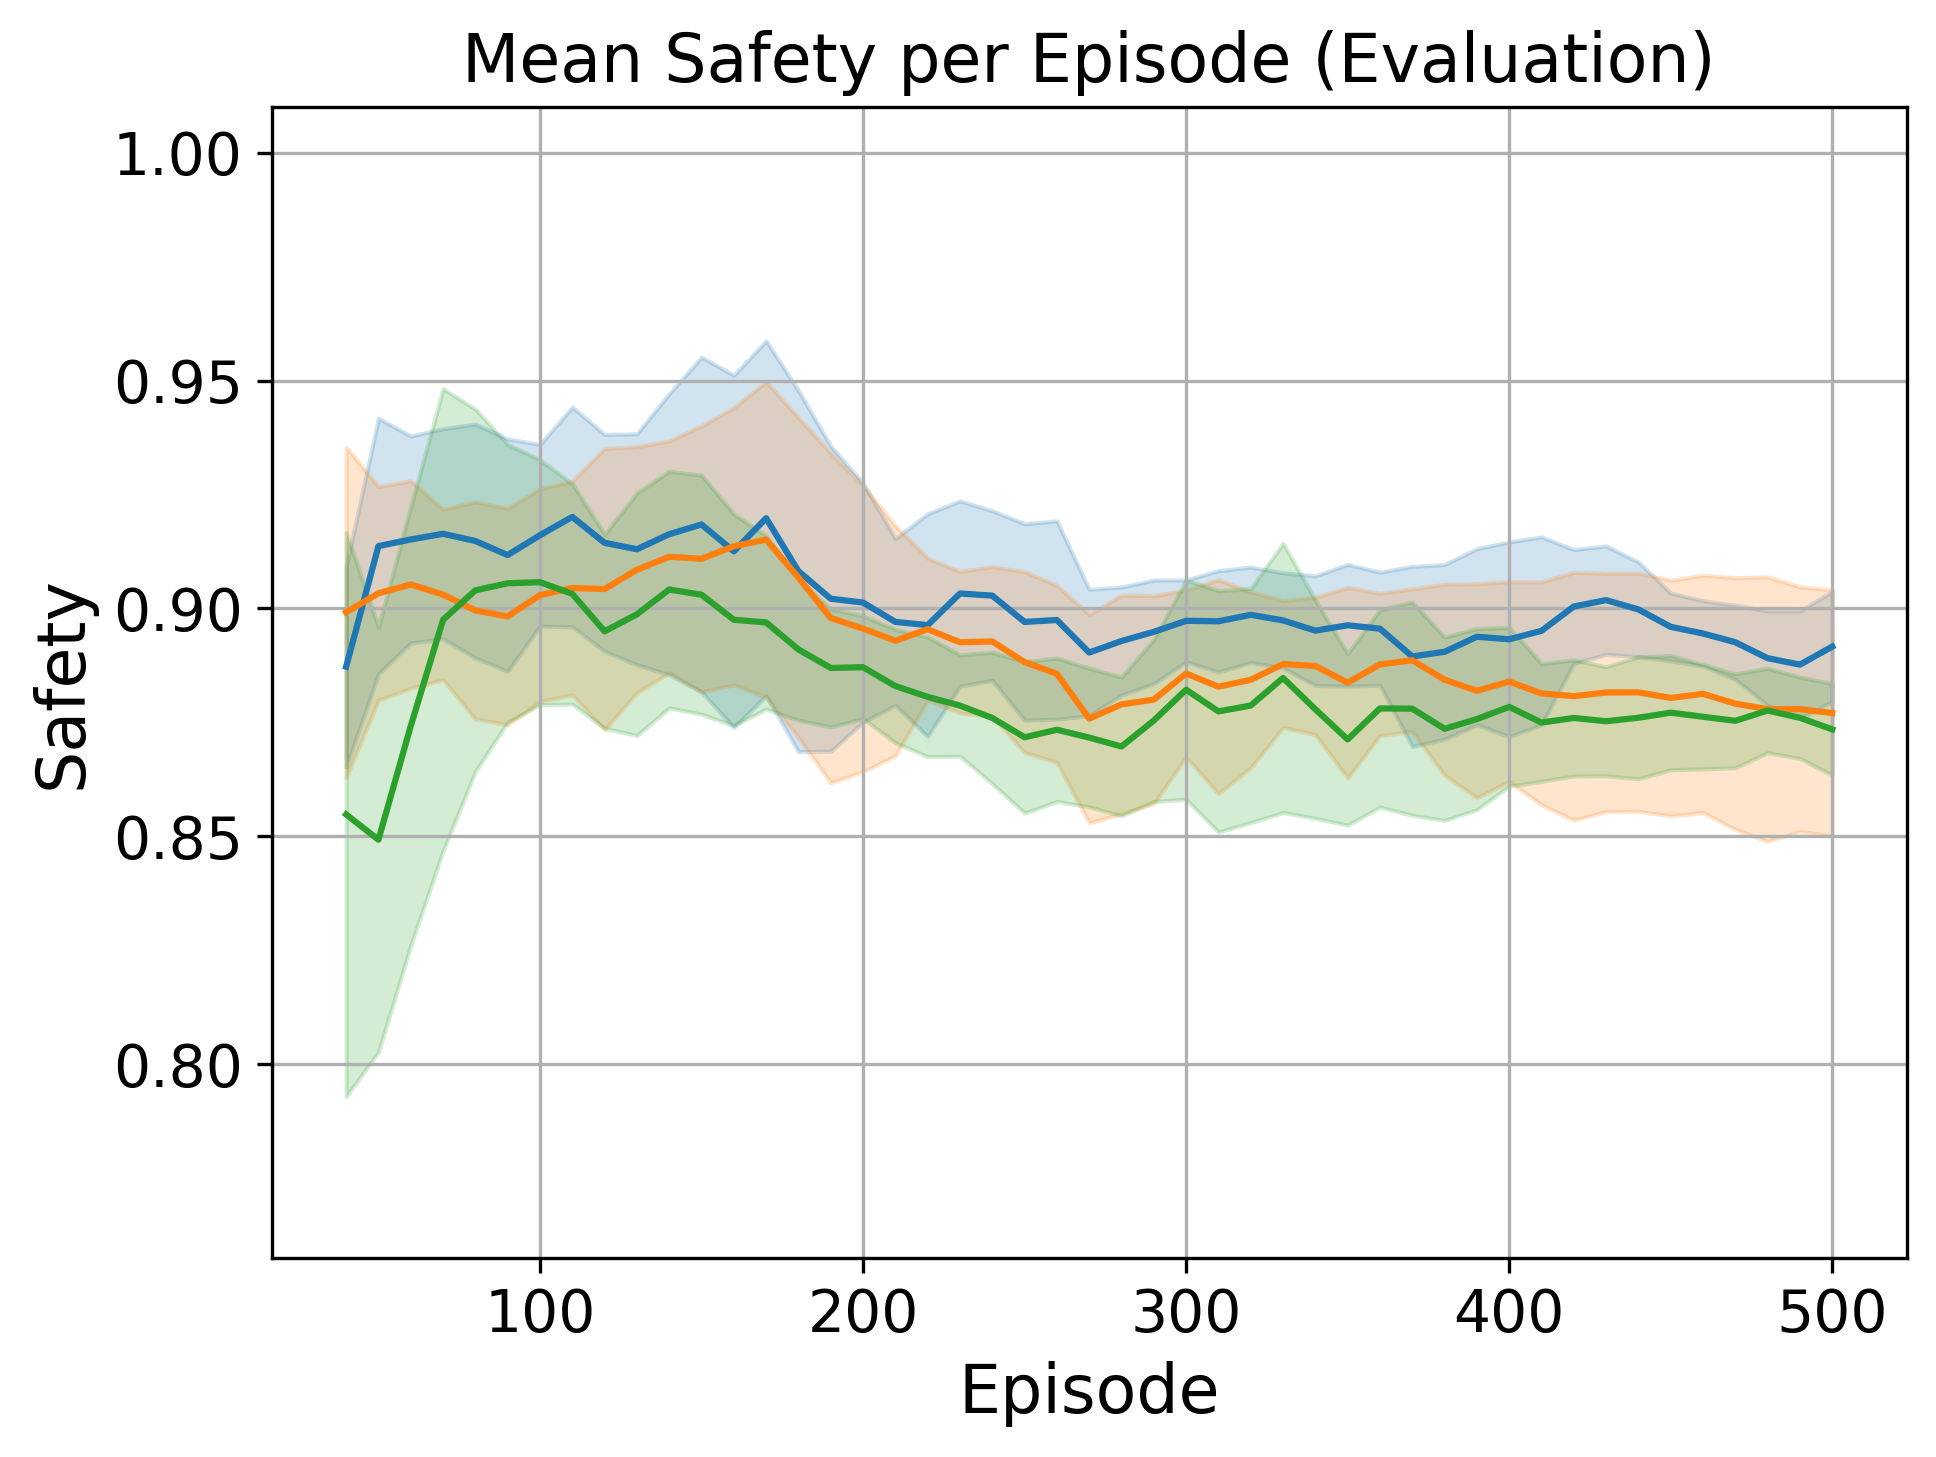
\includegraphics[width=\textwidth]{Experiments/images/cartsafe/safety_DQN_greedy_cartsafe.png}
        \vspace{0.3em}

        \textbf{(c)}
        \label{fig:cartsafe_dqn:sub3}
    \end{minipage}

    \vspace{10pt}

    % Second row: On-policy, epsilon-greedy
    \begin{minipage}[b]{0.32\textwidth}
        \centering
        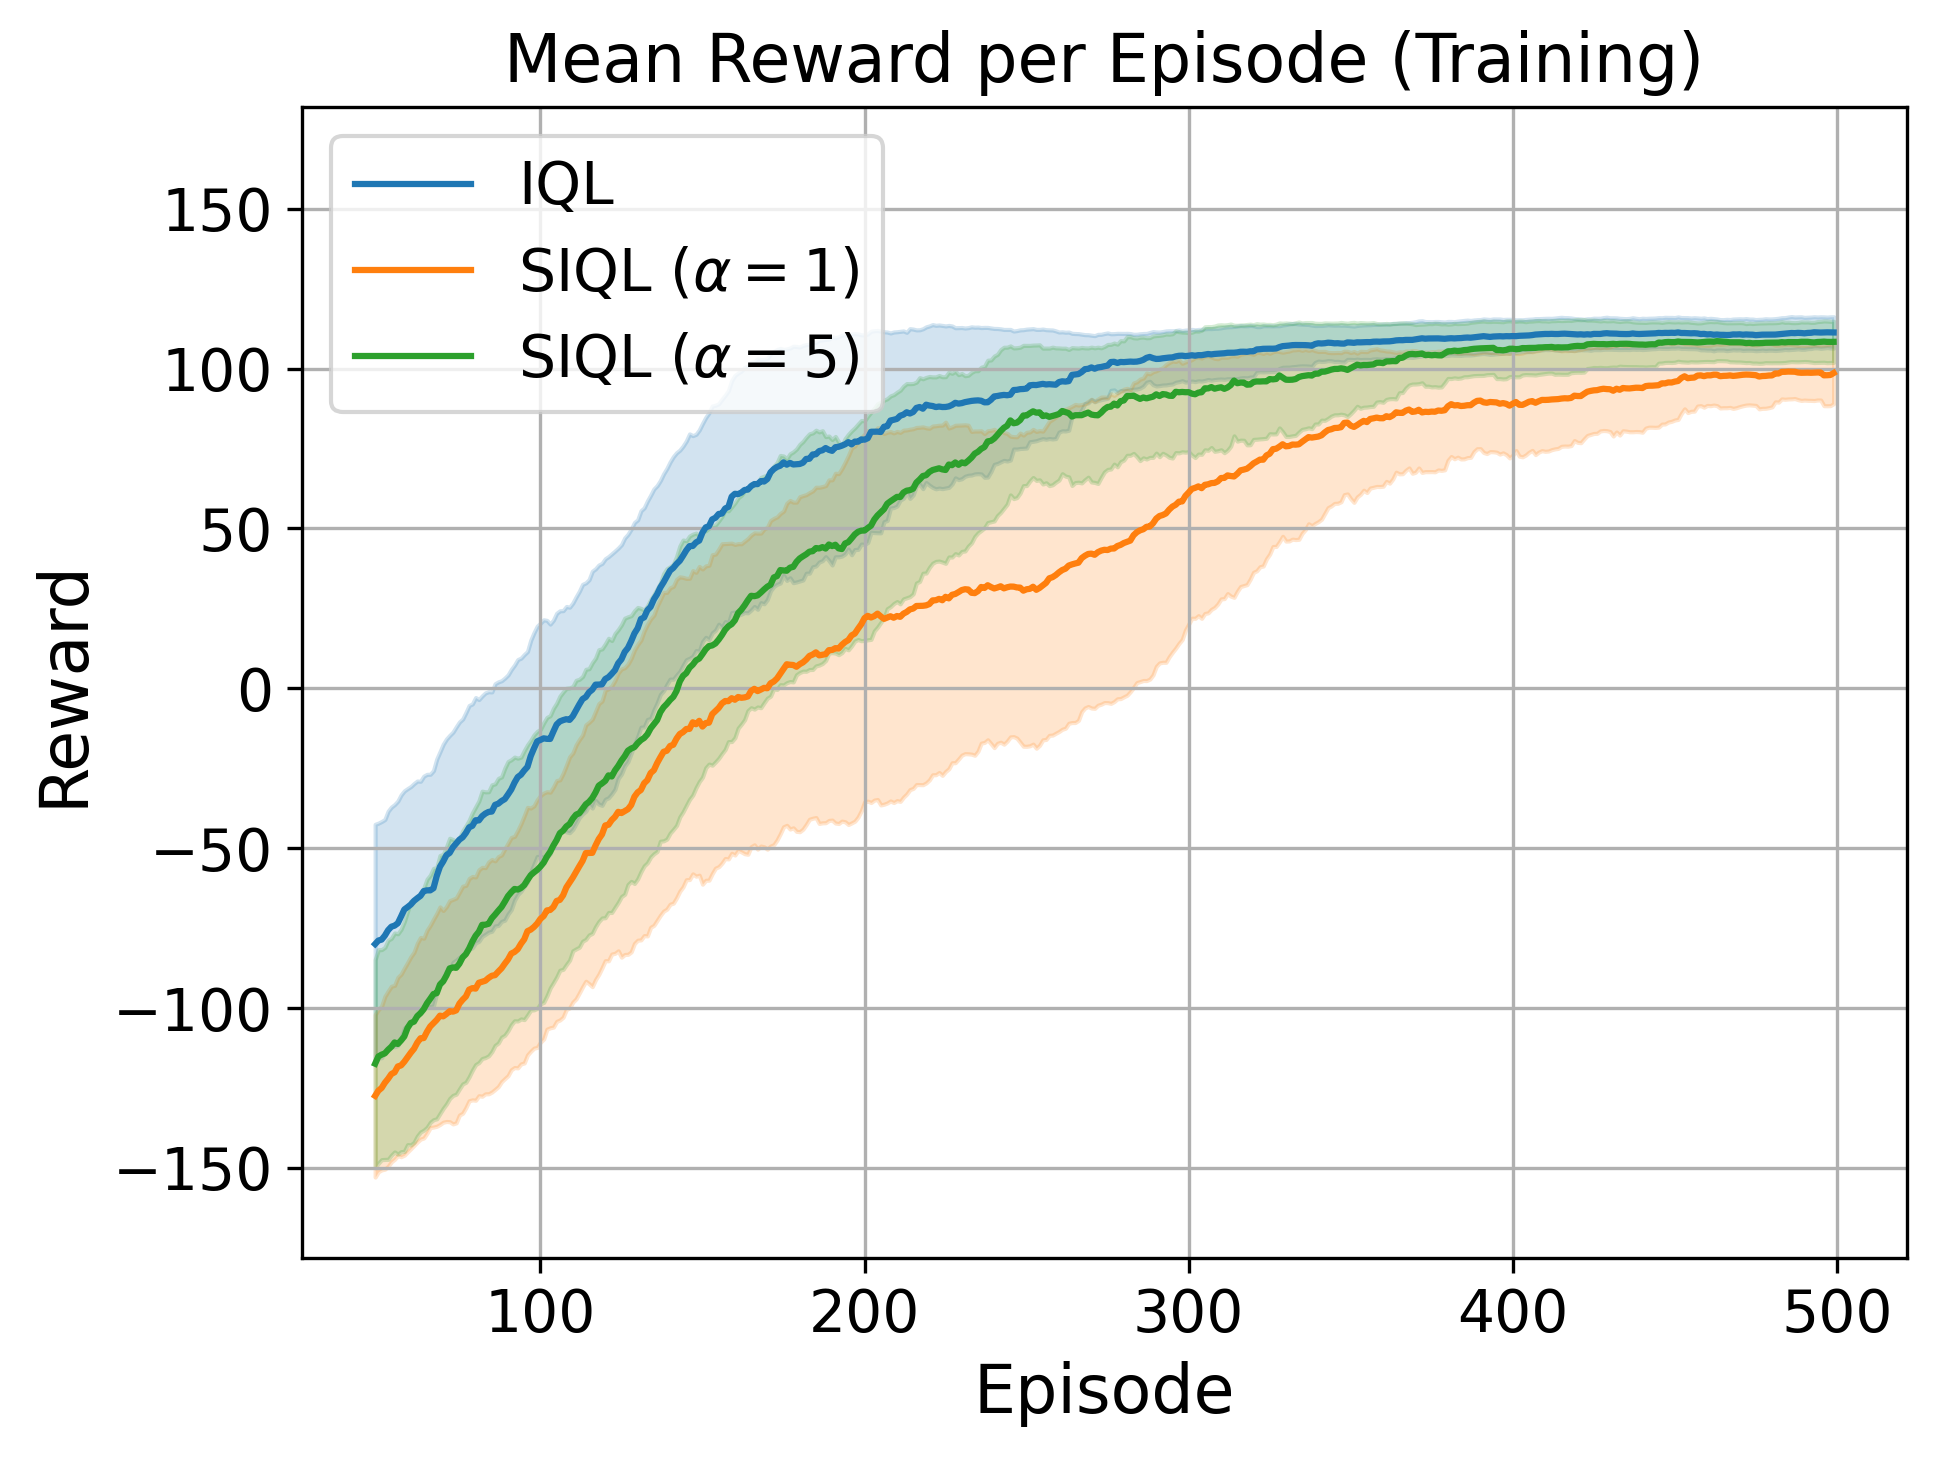
\includegraphics[width=\textwidth]{Experiments/images/cartsafe/training_SARSA_greedy_cartsafe.png}
        \vspace{0.3em}

        \textbf{(d)}
        \label{fig:cartsafe_dqn:sub4}
    \end{minipage}
    \hfill
    \begin{minipage}[b]{0.32\textwidth}
        \centering
        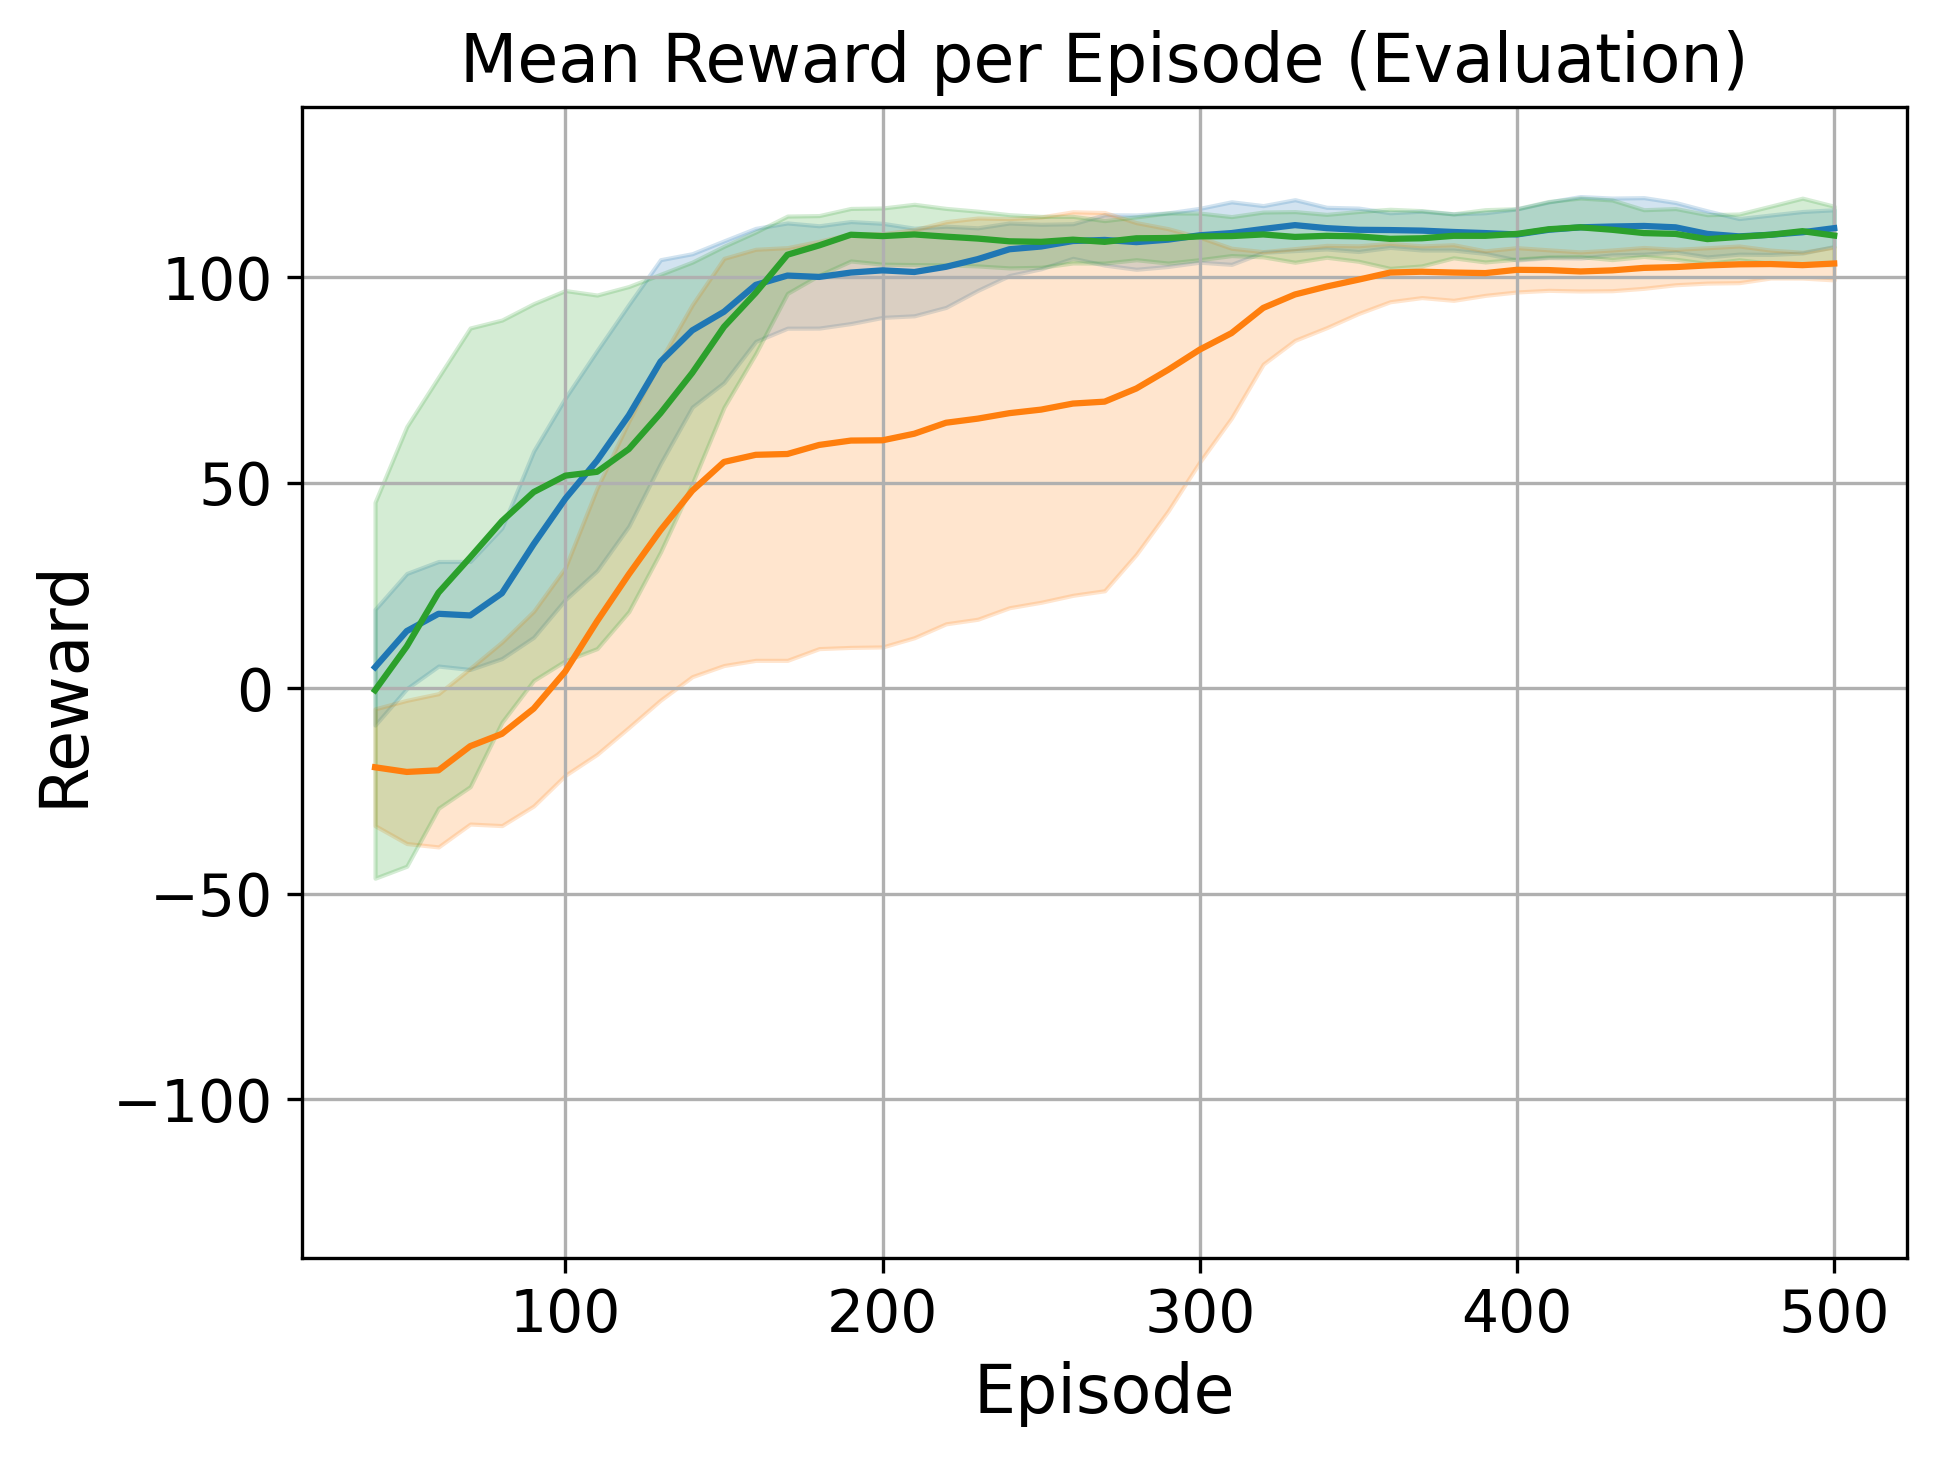
\includegraphics[width=\textwidth]{Experiments/images/cartsafe/eval_SARSA_greedy_cartsafe.png}
        \vspace{0.3em}

        \textbf{(e)}
        \label{fig:cartsafe_dqn:sub5}
    \end{minipage}
    \hfill
    \begin{minipage}[b]{0.32\textwidth}
        \centering
        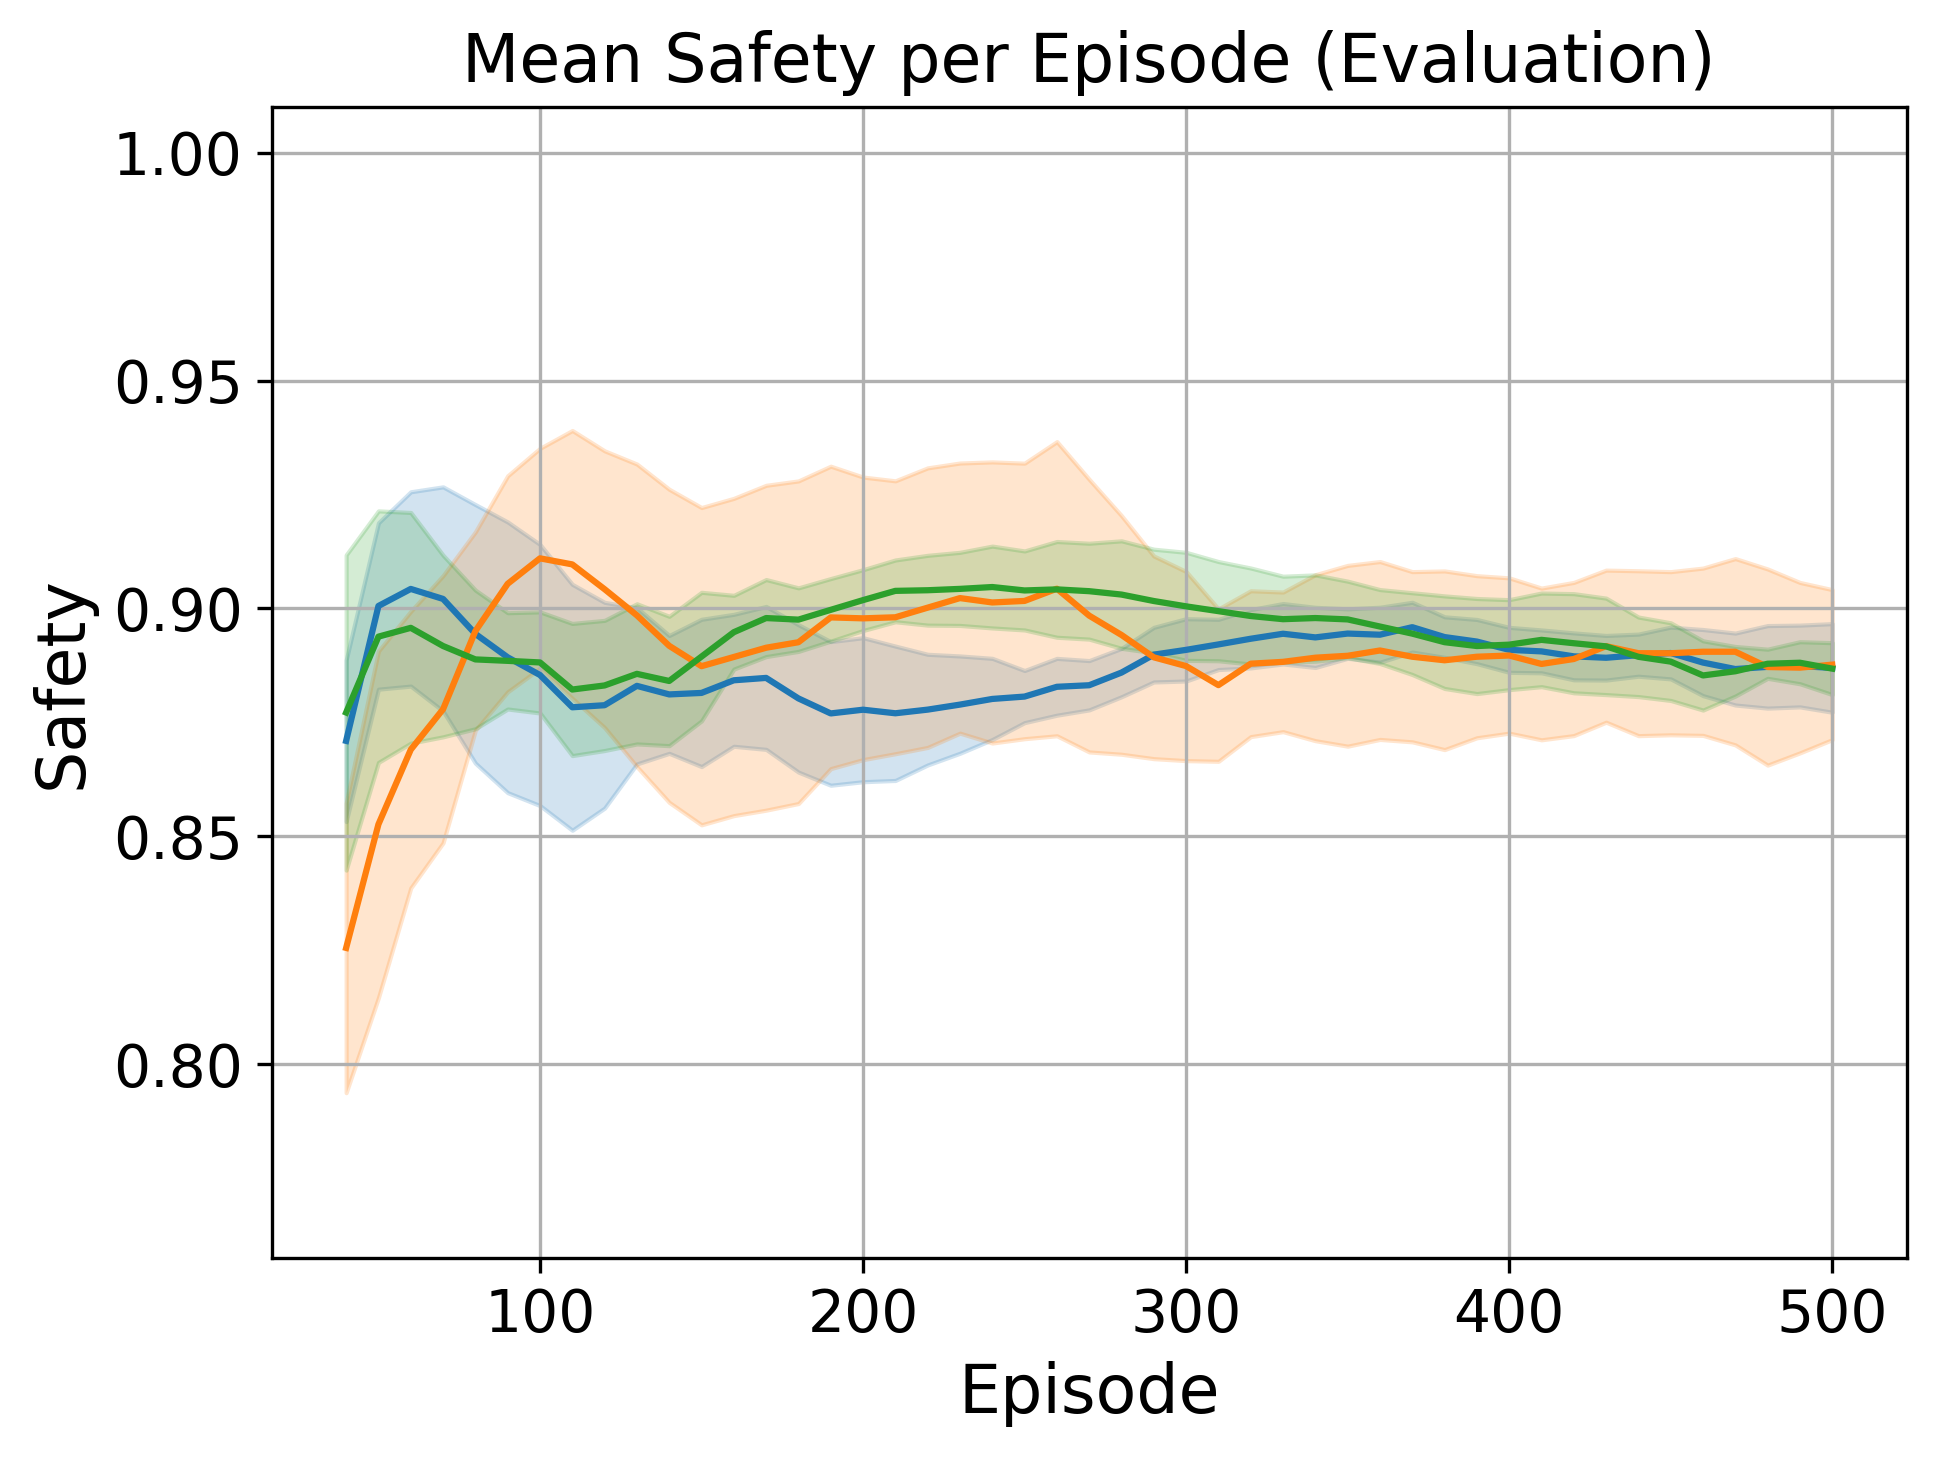
\includegraphics[width=\textwidth]{Experiments/images/cartsafe/safety_SARSA_greedy_cartsafe.png}
        \vspace{0.3em}

        \textbf{(f)}
        \label{fig:cartsafe_dqn:sub6}
    \end{minipage}

    \vspace{10pt}

    % Third row: Off-policy, softmax
    \begin{minipage}[b]{0.32\textwidth}
        \centering
        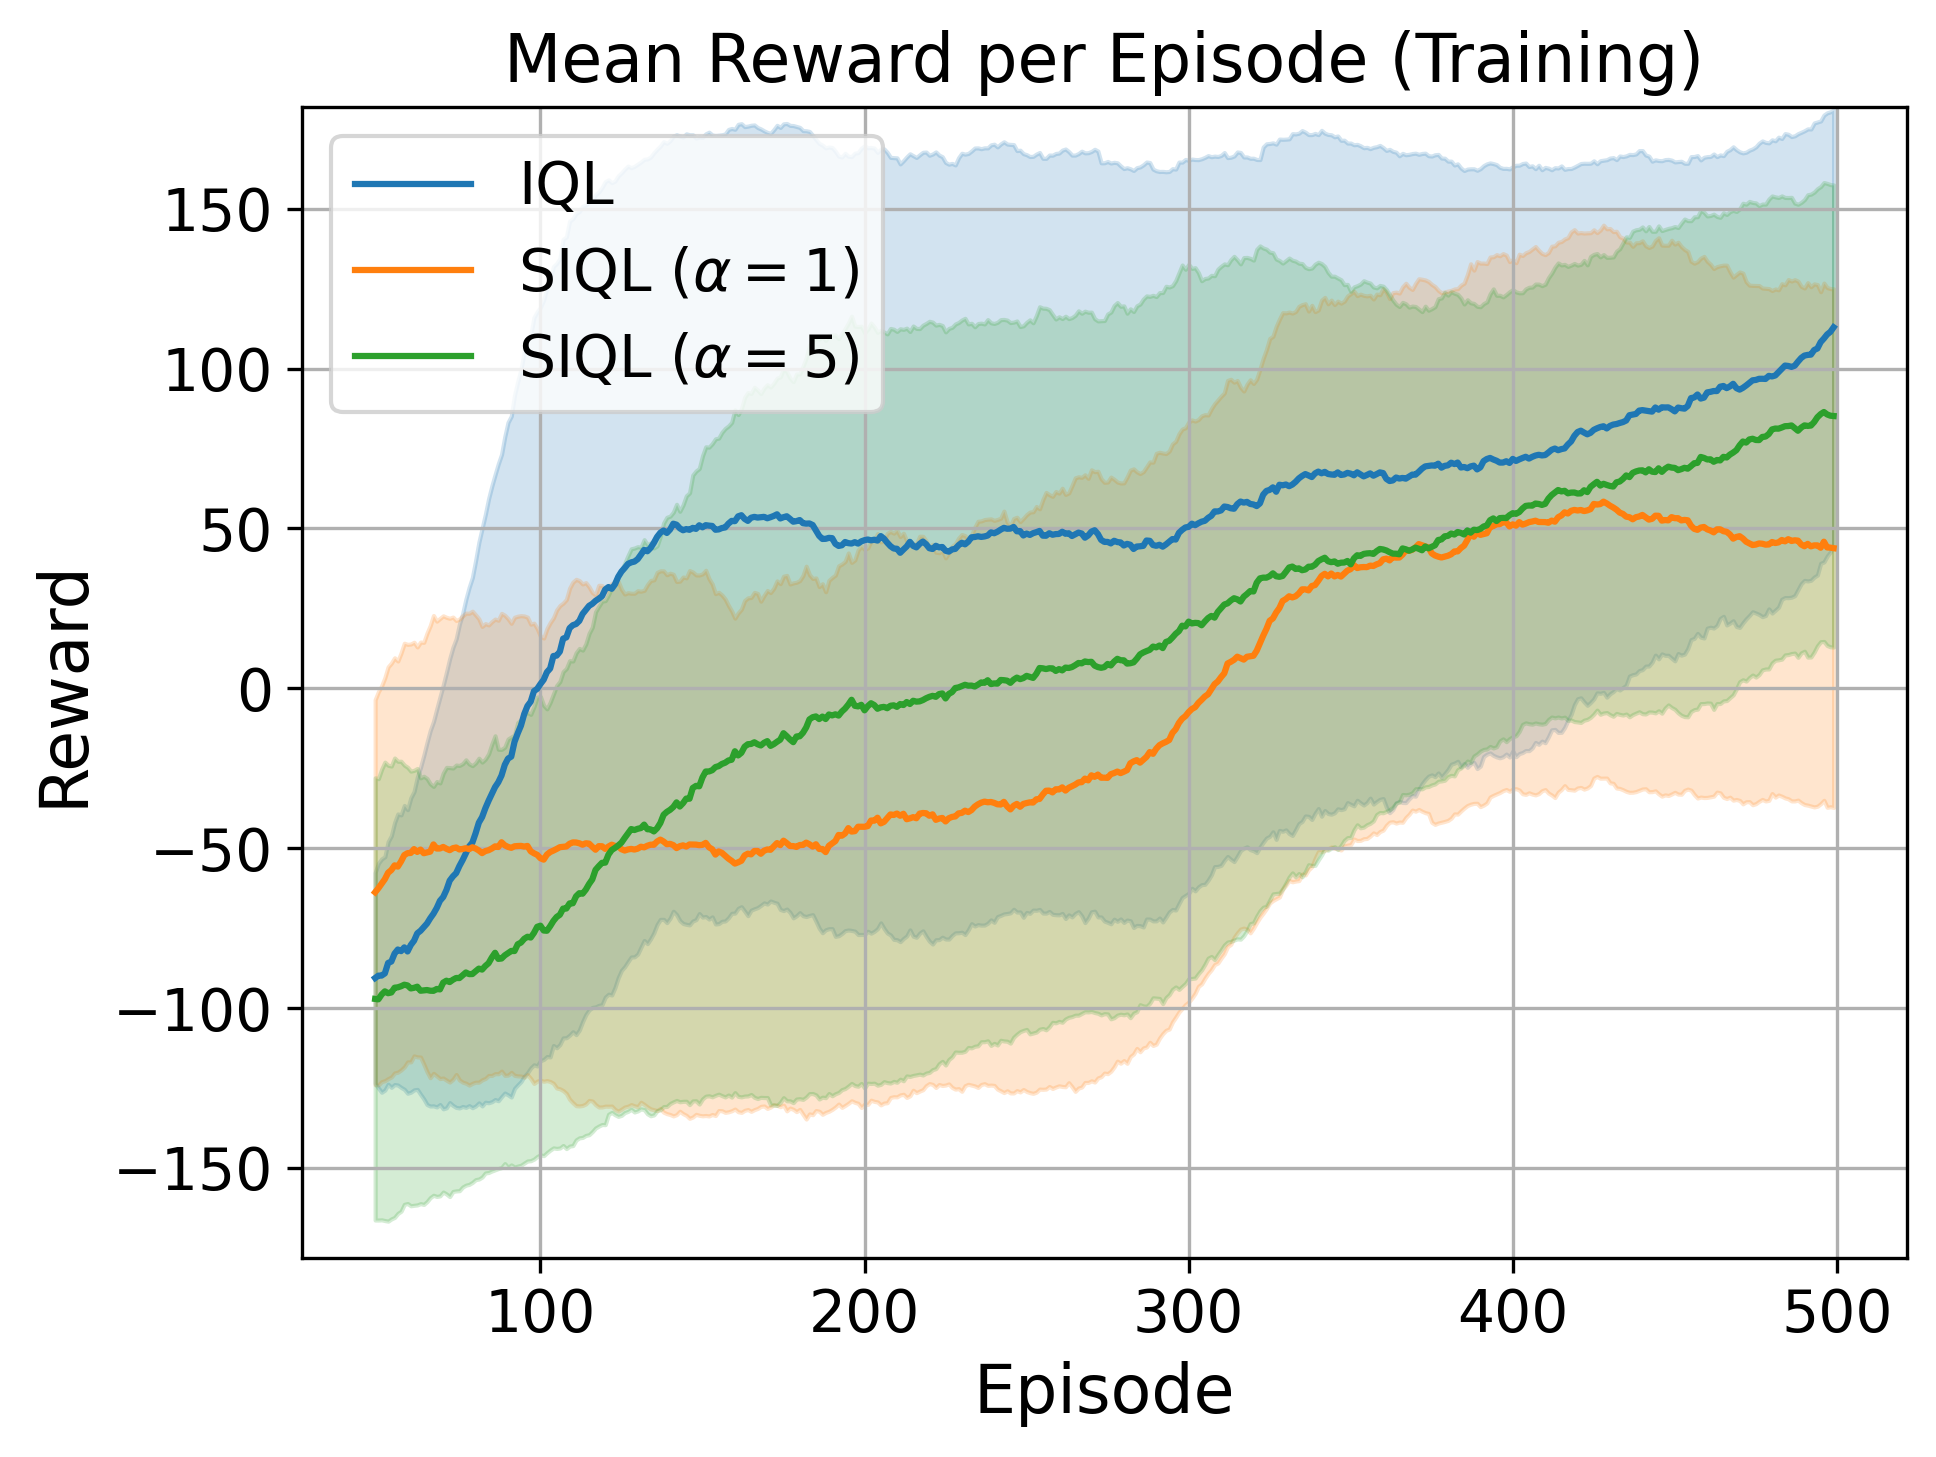
\includegraphics[width=\textwidth]{Experiments/images/cartsafe/training_DQN_softmax_cartsafe.png}
        \vspace{0.3em}

        \textbf{(g)}
        \label{fig:cartsafe_dqn:sub7}
    \end{minipage}
    \hfill
    \begin{minipage}[b]{0.32\textwidth}
        \centering
        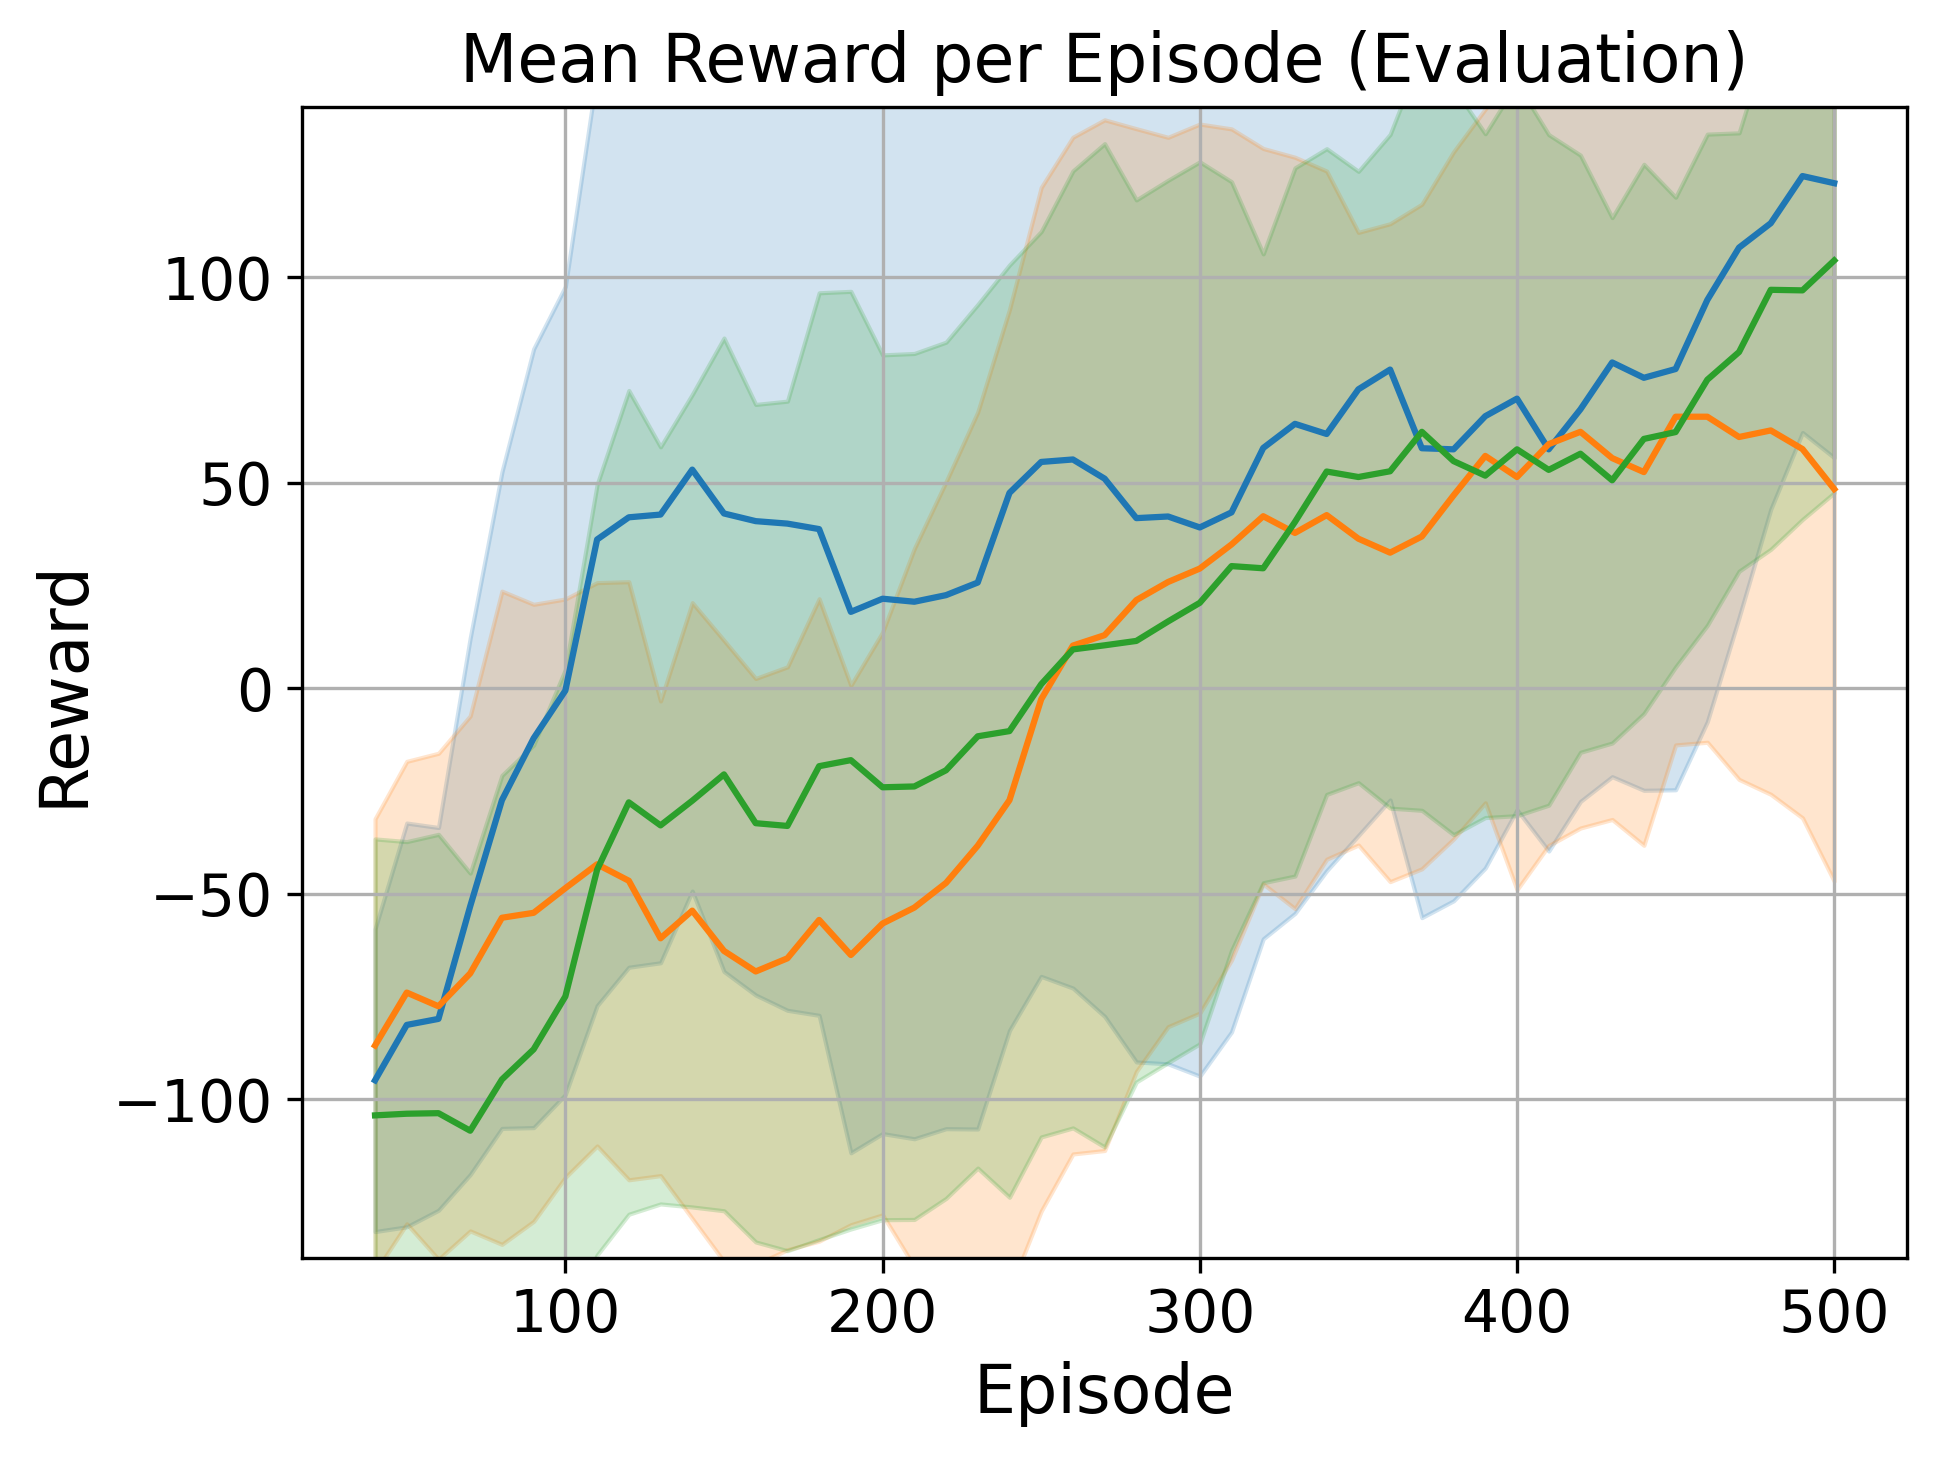
\includegraphics[width=\textwidth]{Experiments/images/cartsafe/eval_DQN_softmax_cartsafe.png}
        \vspace{0.3em}

        \textbf{(h)}
        \label{fig:cartsafe_dqn:sub8}
    \end{minipage}
    \hfill
    \begin{minipage}[b]{0.32\textwidth}
        \centering
        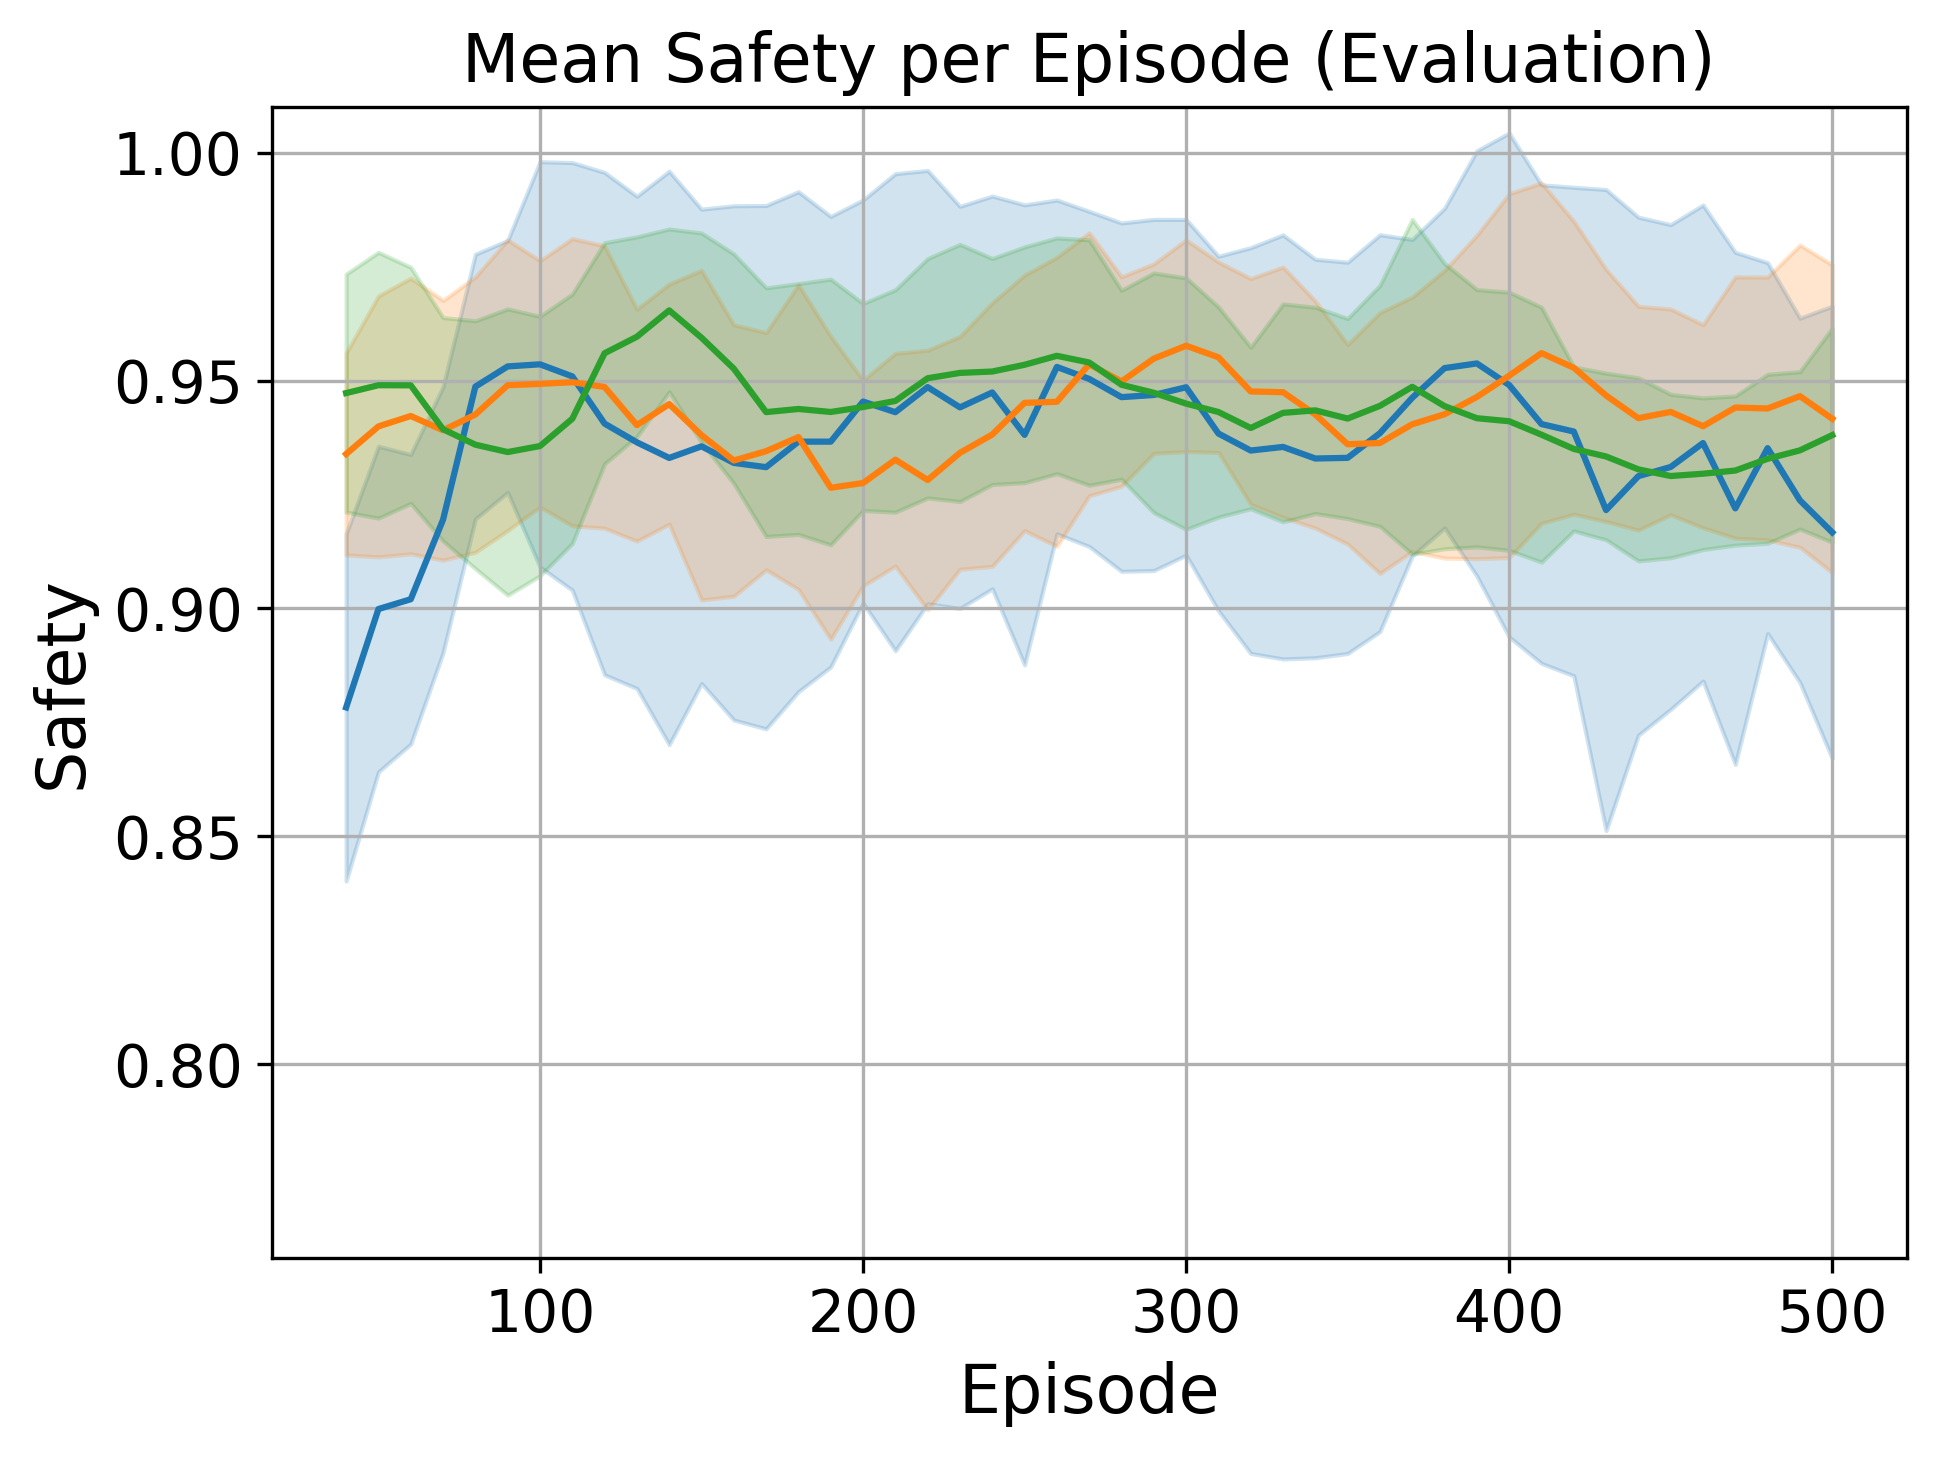
\includegraphics[width=\textwidth]{Experiments/images/cartsafe/safety_DQN_softmax_cartsafe.png}
        \vspace{0.3em}

        \textbf{(i)}
        \label{fig:cartsafe_dqn:sub9}
    \end{minipage}

    \vspace{10pt}

    % Fourth row: On-policy, softmax
    \begin{minipage}[b]{0.32\textwidth}
        \centering
        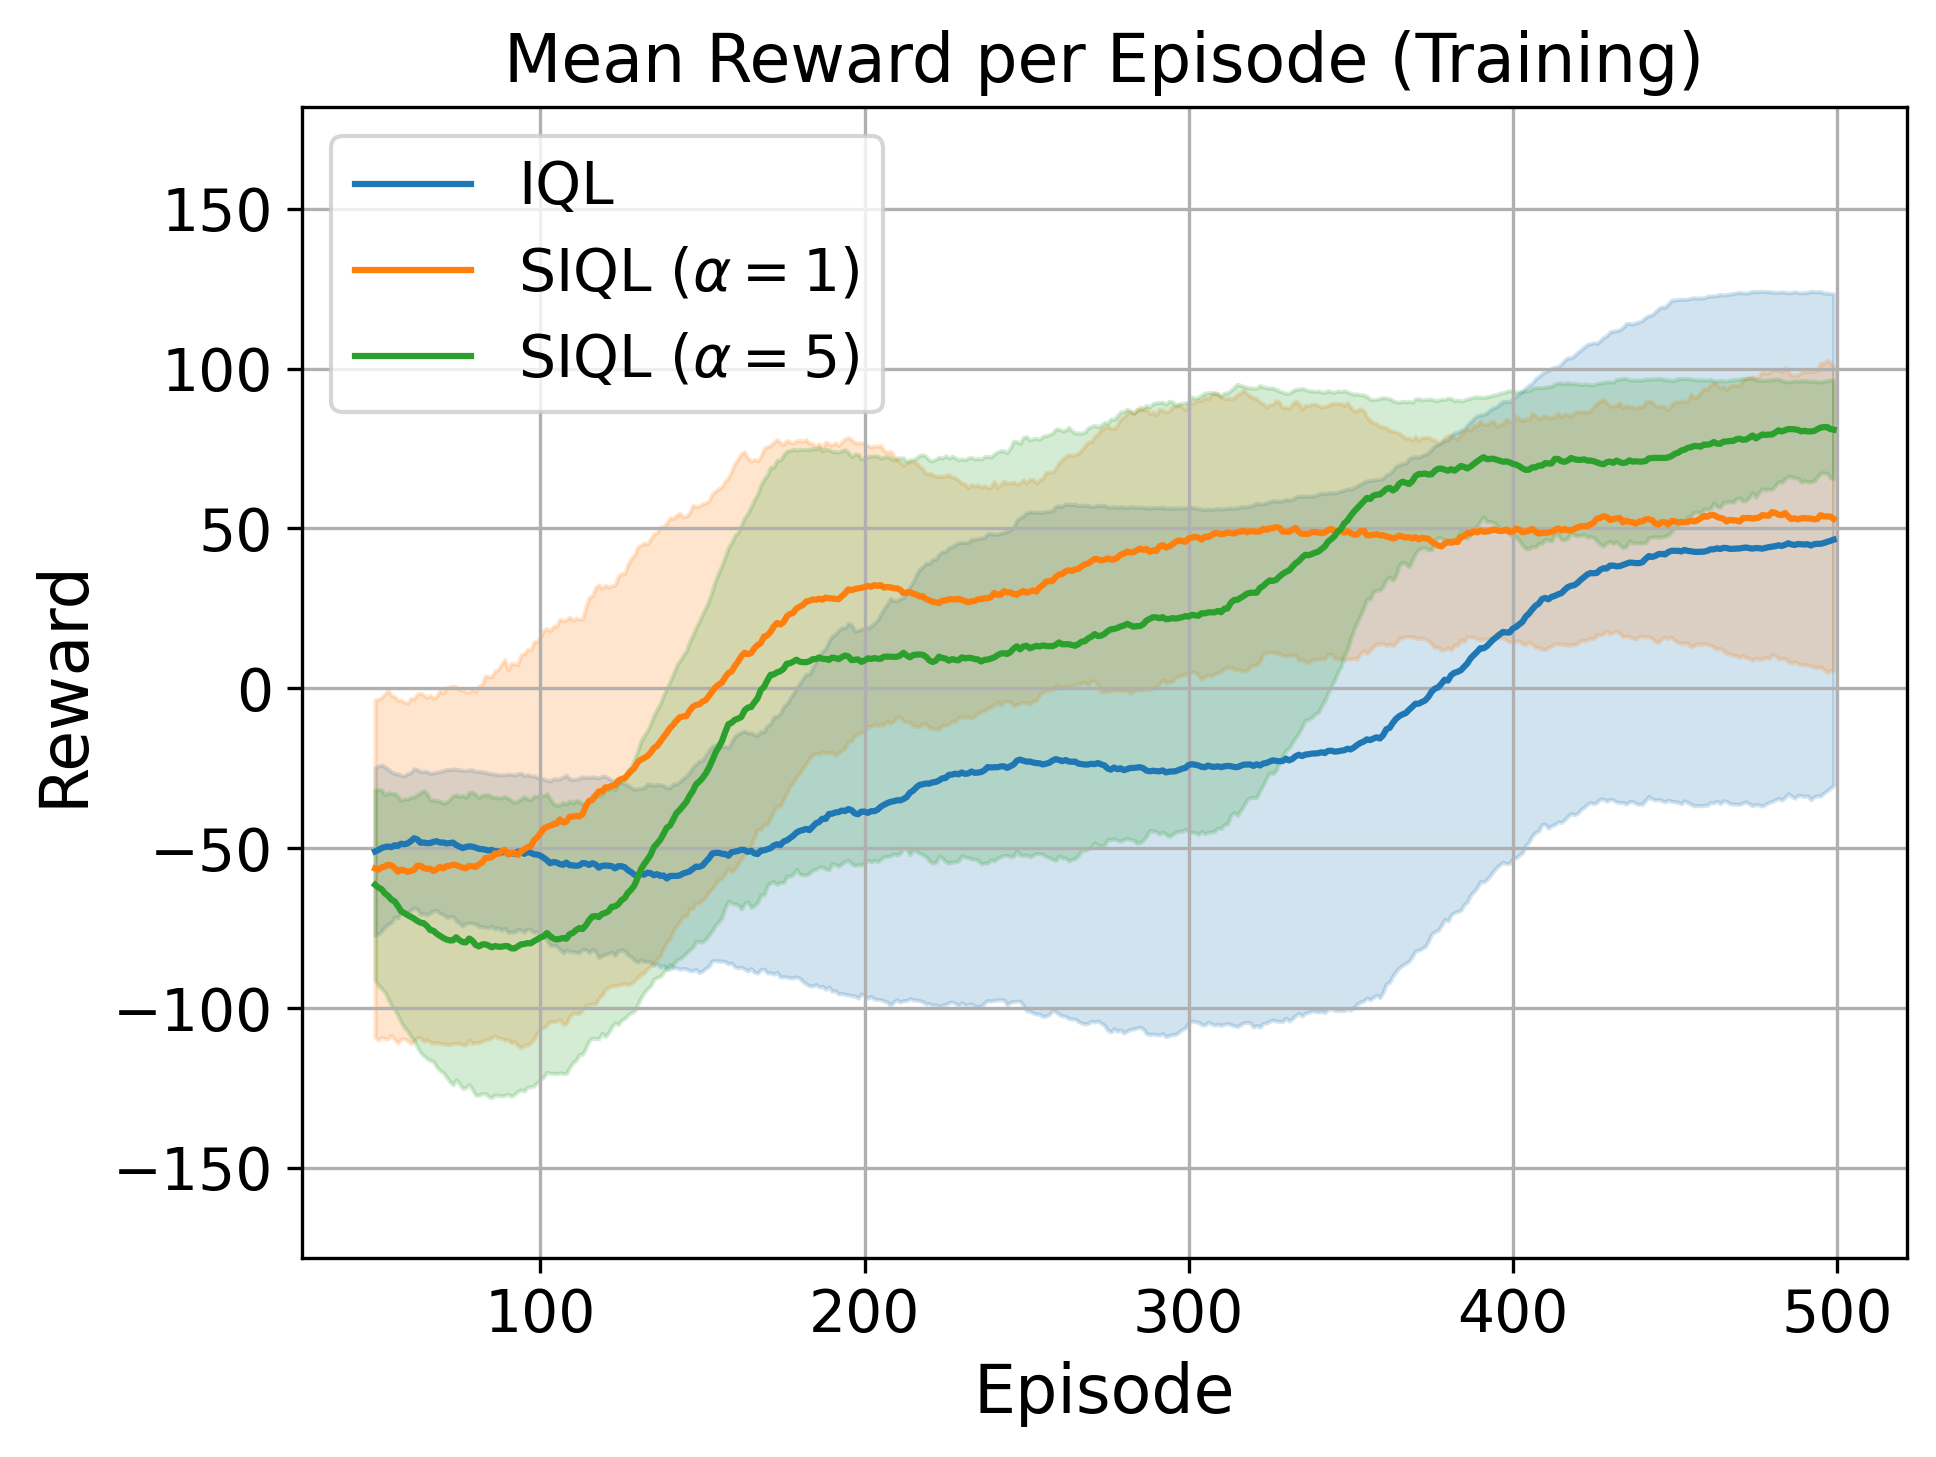
\includegraphics[width=\textwidth]{Experiments/images/cartsafe/training_SARSA_softmax_cartsafe.png}
        \vspace{0.3em}

        \textbf{(j)}
        \label{fig:cartsafe_dqn:sub10}
    \end{minipage}
    \hfill
    \begin{minipage}[b]{0.32\textwidth}
        \centering
        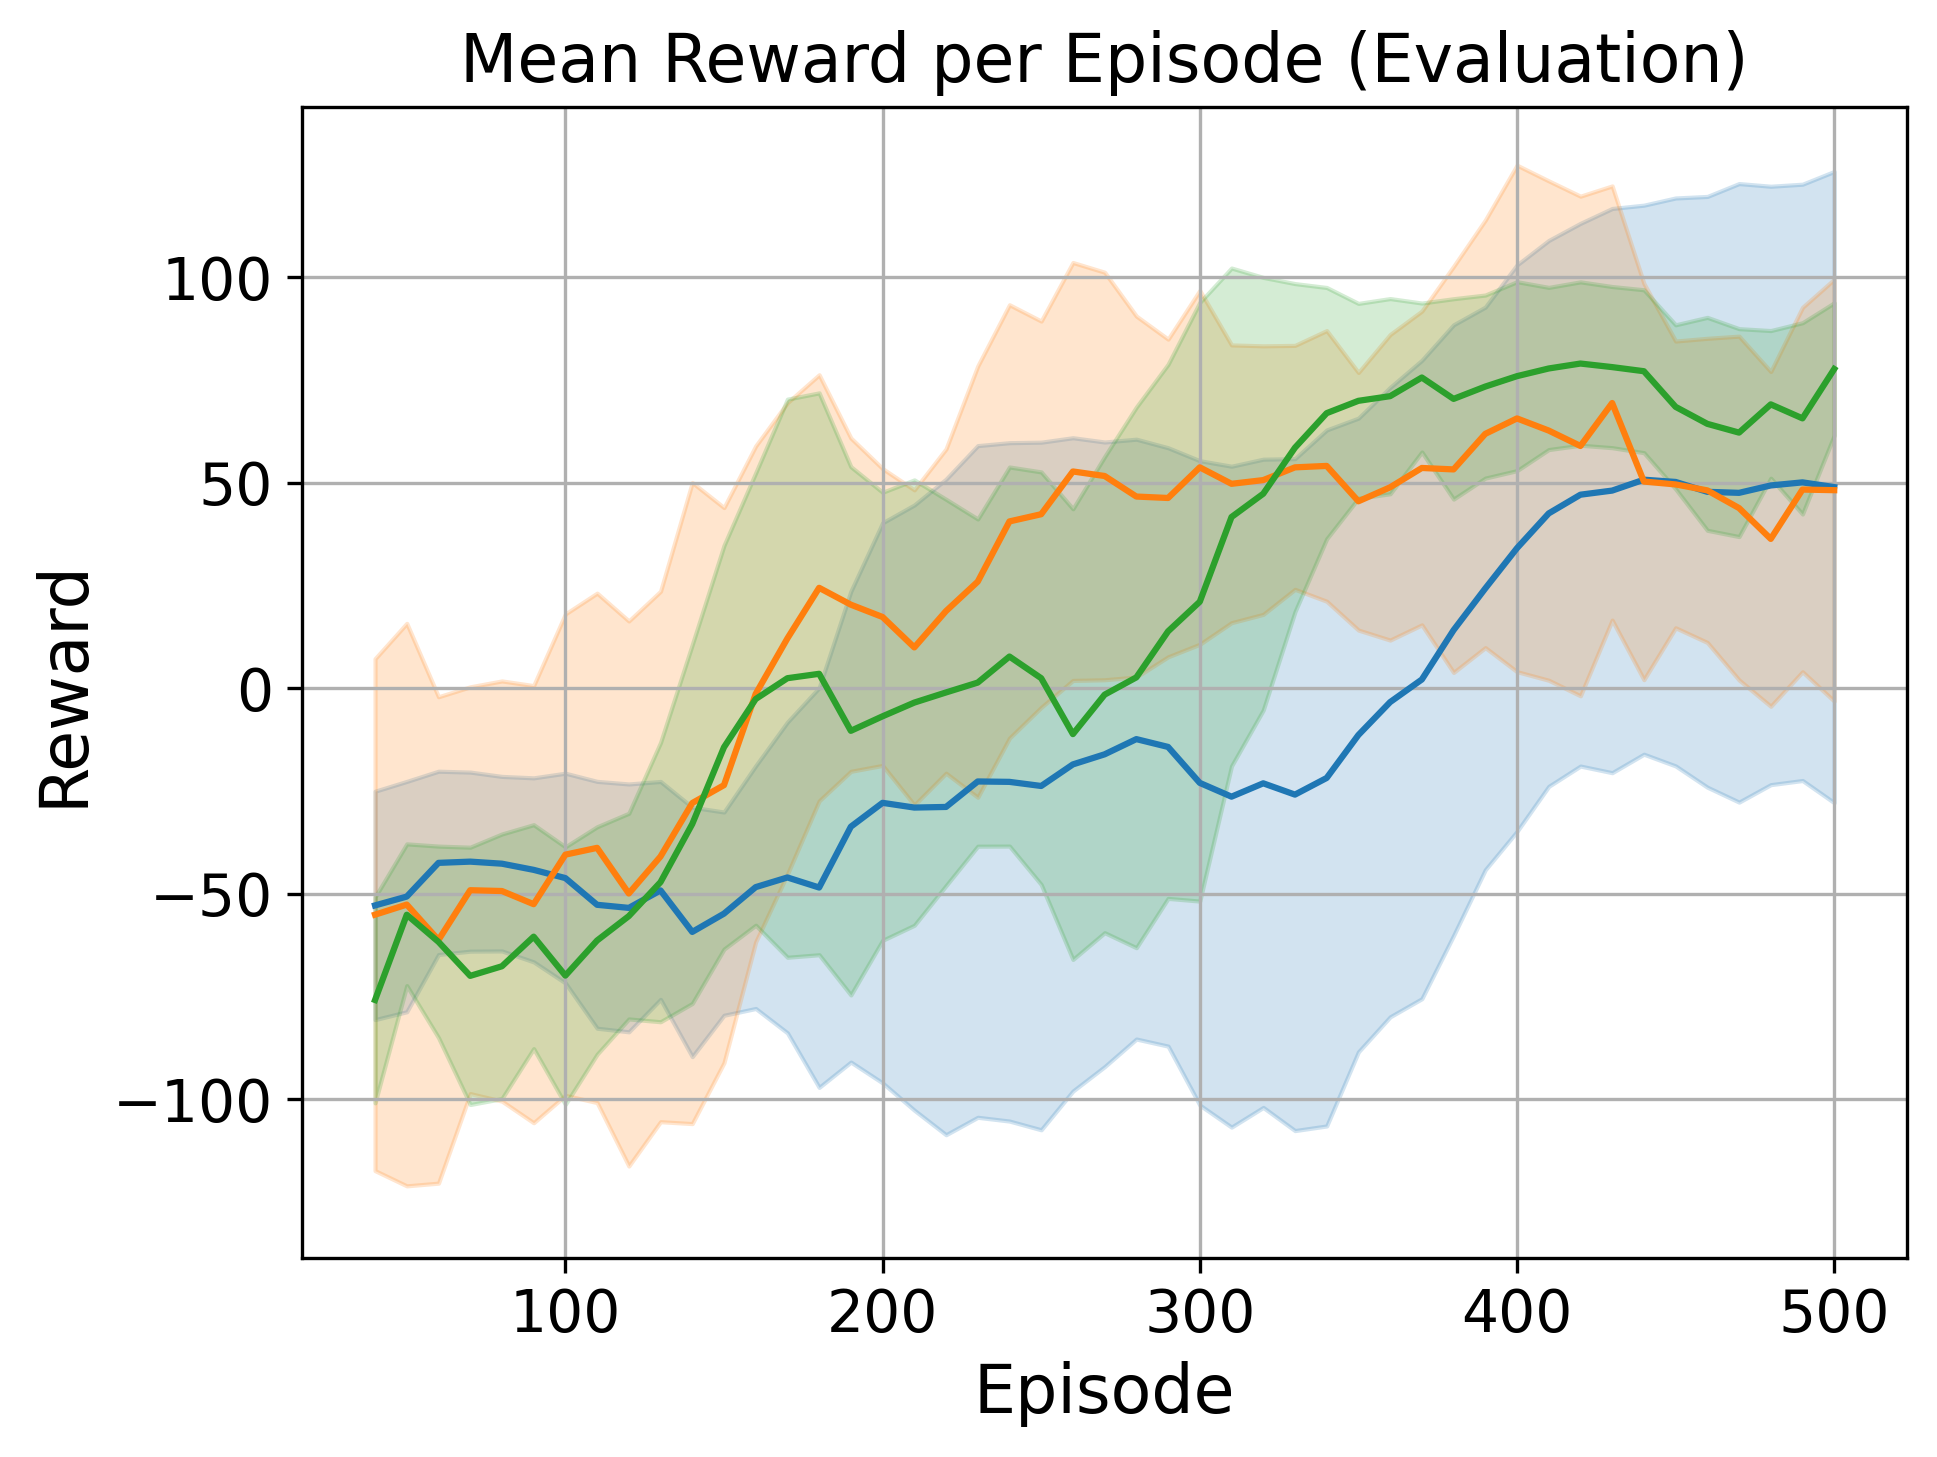
\includegraphics[width=\textwidth]{Experiments/images/cartsafe/eval_SARSA_softmax_cartsafe.png}
        \vspace{0.3em}

        \textbf{(k)}
        \label{fig:cartsafe_dqn:sub11}
    \end{minipage}
    \hfill
    \begin{minipage}[b]{0.32\textwidth}
        \centering
        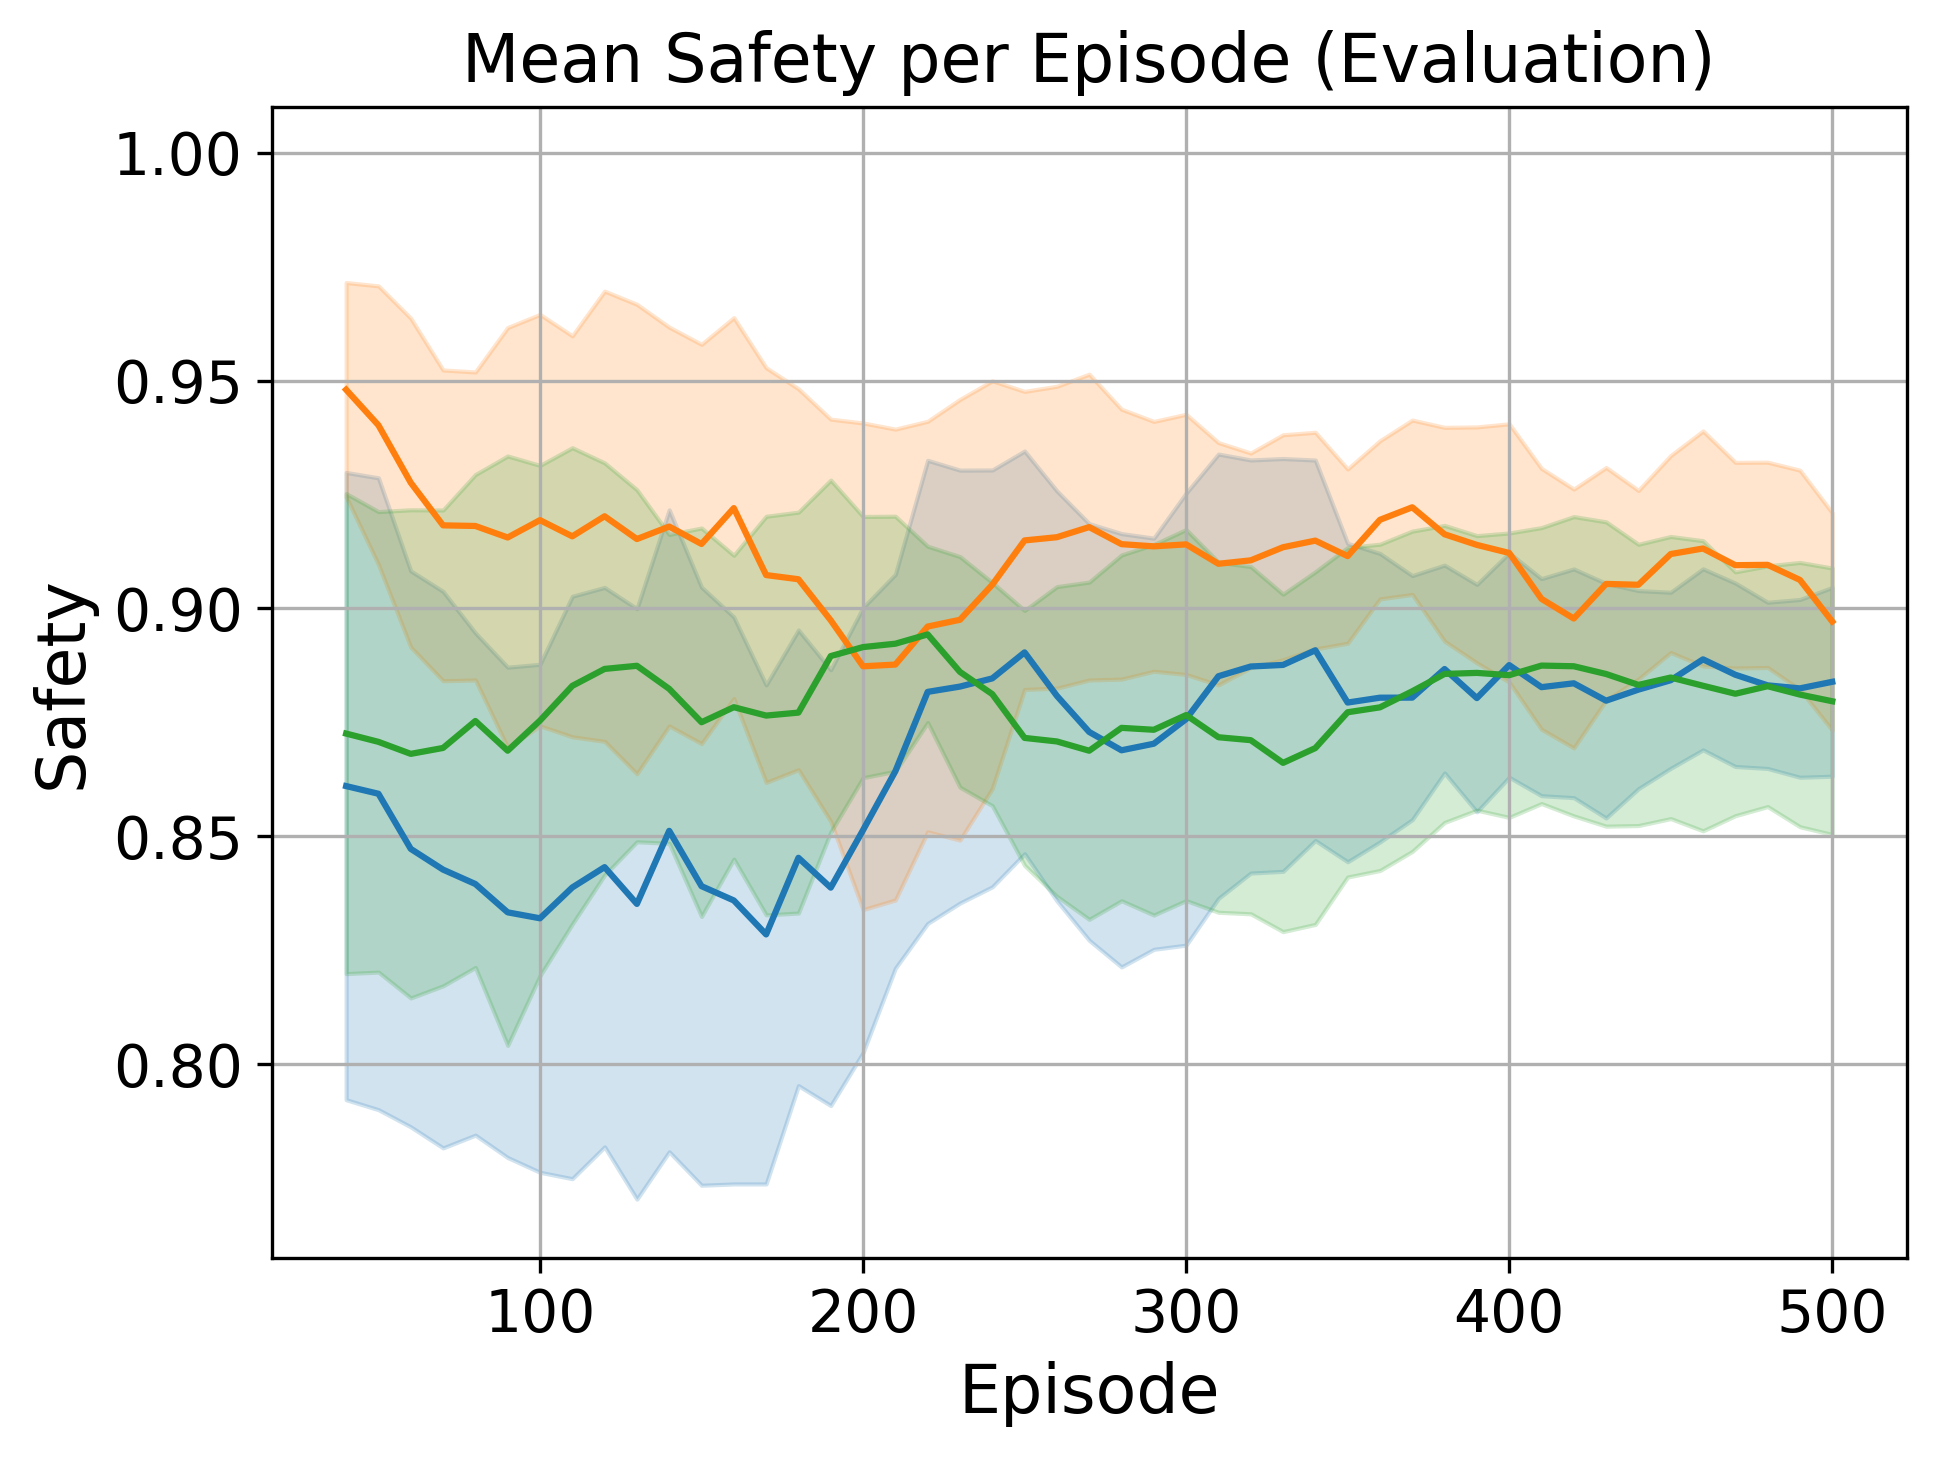
\includegraphics[width=\textwidth]{Experiments/images/cartsafe/safety_SARSA_softmax_cartsafe.png}
        \vspace{0.3em}

        \textbf{(l)}
        \label{fig:cartsafe_dqn:sub12}
    \end{minipage}

    % Figure caption
    \caption[Single-agent Results for \textit{CartSafe} (PLTD agents).]{Training, evaluation and safety results for \textit{CartSafe} for on- and off-policy DQN-based agents with different exploration strategies: \textit{top row:} off-policy, $\epsilon$-greedy; \textit{top middle row:} on-policy, $\epsilon$-greedy; \textit{bottom middle row:} off-policy, softmax; and \textit{bottom row:} on-policy, softmax. The lines represent the mean and the shadow the standard deviation over 3 seeds.}
    \label{fig:cartsafe_dqn}
\end{figure*}

Before testing the two shielded multi-agent DQN-based algorithms (SIQL and SPSQL), it is imperative to first test whether or not PLTD (ProbLog-shielded DQN) works as well as vanilla DQN for environments with constraints, and how it compares to PLPG (ProbLog-shielded PPO). Additionally, it would be useful to verify that the custom PLPG code works for single agent settings before attempting multi-agent experiments.

\textit{CartSafe} is modification of OpenAI Gym's classical control problem \textit{CartPole} \citep{brockman1606.01540} with simple constraints inspired by \citet{jemaw2019}. The problem has the following elements: the environment consists of a rod attached to a box or cart at one end and is allowed to freely swing around the attachment point. This setup exists in a bounded 2-dimensional real space with a set width and an active physics simulation. At each time step, the agent has two actions: accelerate the cart to the left or to the right. The agent observes the cart's position, velocity, the angular velocity of the rod and the angle of the rod in radians. The goal is to actively balance the rod upright without leaving the bounds of the environment. The agent receives a reward at each time step based on the angle of the pole ($\theta_{pole}$) with respect to vertical: $r^t=1$ if $-15^\circ\leq\theta_{pole}\leq15^\circ$ and $r^t=-1$ otherwise. The environment terminates when a maximum number of steps ($t_{max}$) are reached or the cart moves off screen. The additional constraints that are added to this setup are such that the cart must not enter the region bounded by the leftmost and rightmost quarters of the environment -- thus the agent must learn to balance the rod near the center of the screen.

The purpose of this experiment is trifold: 
\begin{enumerate}
    \item To test whether the PLPG and ProbLog shield implementations adequately work on a common RL task with a continuous state space;
    \item To verify the ideas of PLTD introduced in Section 3.2 and its implementation to see whether it would help (or at least does not hurt) the ability of a DQN agent converging to a good and safe policy;
    \item To explore the possibilities in terms of exploration and on/off-policy strategies to see how they affect performance and safety of PLTD agents.
\end{enumerate}

\subsection{Experimental conditions}
The maximum length of each episode was set to $t_{max}=200$ with 500 training episodes. The agents are evaluated every 10 episodes. Each algorithm was re-run with 5 different seeds each and their aggregated results are discussed below. The PPO and DQN parameters were minimally hand-tuned and can be found in Table~\ref{table:hyperparams} in Appendix~\ref{appsec:hyperparams}. The PPO agents were shielded with safety penality coefficient $\alpha\in\{0.5,1.0,2.0\}$. The DQN-based algorithms were tested by varying the following aspects: on-policy vs.\ off-policy, $\epsilon$-greedy vs. softmax exploration (paired with greedy and softmax exploitation policies respectively) and whether they are shielded (SIQL with safety coefficient $\alpha\in\{1.0,5.0\}$) or not (IQL).


% \begin{figure}[h]
%     \centering
%     \fbox{
%     \includegraphics[width=0.3\linewidth]{Experiments/images/cartsafe/cartsafe_env.png}}
%     \caption[Starting Configuration for \textit{CartSafe}.]{Example starting configuration for \textit{CartSafe}. The `cart' is the black box that the agent controls, the brown rectangle is a `pole' that pivots around the purple attachment point. The regions to the right and left of the red vertical lines are the constrained regions ($\pm1$ unit away from the center, with a maximal width of the environment at 4.8 units).}
%     \label{fig:cartsafe_env}
% \end{figure}

\subsection{Shield construction}
A simple shield that aims to satisfy the constraints outlined in the task description can be constructed as follows:
\begin{lstlisting}[language=Prolog, caption={Shield for soft constraint satisfaction for \textit{CartSafe}.}, label={shield:cartsafe}]
% actions
action(0)::action(left);
action(1)::action(right).

% sensors
sensor_value(0)::sensor(cost).
sensor_value(1)::sensor(xpos).
sensor_value(2)::sensor(left).
sensor_value(3)::sensor(right).

% constraints
unsafe_next :- action(X), sensor(X), 
               sensor(cost), sensor(xpos).
safe_next :- \+unsafe_next.
\end{lstlisting}

The actions correspond to moving the cart to the left or right. The sensors here correspond to (in order) whether or not the current state is within a constrained region (Boolean value), the distance from the center on the $x$-axis normalized between 0 and 1 (such that it is 0 when the cart is in the middle, and 1 when it is at the right or left edges of the screen), and whether the cart is on the left side or right side of the screen (Boolean value). The constraint can be interpreted as \textit{it is unsafe if an action is taken towards some side X, the cart is on side X, the current state is in the constrained region, and the x-position is sufficiently large.} 




This means that if the cart is within the permissible central region of the environment, the safety probability of the next action is computed as $(\texttt{sensor(cost)}=0)\implies(\texttt{safe\_next}=1)$, and the policy remains unchanged. If the cart is too far right, outside the permissible region, it is unsafe to move the cart towards the right. The \textit{right} action gets progressively more unsafe as the cart gets further to the right. The safe policy will proportionally favor the left action as a result. Analogous behavior occurs if the cart is too far left instead of right.

Note that this also means that the agent is \textit{already} within the constrained region (specifically, at the edge of the region) when the shield takes effect -- this can be easily solved by instead having a predicate that looks at whether the \textit{next} step will be impermissible given an action, rather than whether is \textit{currently} is in such a state. However, this should not significantly alter the behavior of the agent in this environment.

Note that $\texttt{sensor(xpos)}$ is the \textit{only} non-Boolean input to this shield. If it not placed in the body of the constraint in line 12, since \texttt{sensor(X)} and \texttt{sensor(cost)} are purely Boolean, the safe policy computation will result in a deterministic behavior in the constrained regions -- \textit{go left if the cart is in the right-hand constrained region with probability 1}, and vice-versa for the left-hand constrained region. Thus, the behavior of the agent act safely immediately and deterministically. The inclusion of $\texttt{sensor(xpos)}$ allows us to experiment with soft constraints -- here, it enforces the idea that it gets linearly worse when travel deeper into the constrained regions.


\subsection{Results: PLTD (Shielded DQN)}

Figure~\ref{fig:cartsafe_dqn} displays training, evaluation and safety results of a variation of PLTD agents. As a reminder, these agents vary in the following aspects: on-policy vs.\ off-policy, $\epsilon$-greedy vs. softmax exploration (paired with greedy and softmax exploitation policies respectively) and whether they are shielded (SIQL with safety coefficient $\alpha\in\{1,5\}$) or not (IQL).

\paragraph{\textit{Shielding}:} First, we may look at whether adding a shield significantly alters the behavior of the agent in this setting. The rightmost column shows the mean safety per episode computed with the CartSafe shield (Shield~\ref{shield:cartsafe}). We see that in general, adding a shield to an agent with either of the tested safety penalty values does not significantly affect its safety, \textit{ceteris paribus}. However, all safety values tend to be quite high, generally above 0.9 with not much improvement after the first $\approx100$ episodes. We also note that the shielded agents do not do \textit{worse} than the unshielded ones. This may hint at the safety constraints being relatively simple to accomplish given the environment goals and algorithms. Thus there is little to no trade-off between reward and safety in this task.

\paragraph{\textit{$\epsilon$-Greedy vs.\ Softmax}:} When looking at the difference between the exploration and exploitation strategies, we see quite a large difference in the variation of results when trained multiple times -- the $\epsilon$-greedy-based algorithms tend to more reliably converge to a good policy (converging around reward $\approx100$), whereas the softmax policies tend to have a much larger standard deviation with less smoothly increasing curves, to policies that generally attain less reward per episode.

\paragraph{\textit{On vs.\ Off-Policy}:} For the $\epsilon$-greedy runs, it is noticeable that the on-policy versions of the algorithms all tends to converge faster than the off-policy ones, reaching around reward~$\approx$~50 in 100 episodes during evaluation versus 200 episodes for off-policy DQN. We do not see the same trend for the softmax policies, it seems that that it does reduce the variance across seeds significantly. There does not seem to be a significant difference in safety between these two conditions. One outlier in this regard is that the off-policy agents with softmax policies are slightly but significantly more safe than all the others.

\paragraph{\textit{PLTD vs.\ PLPG}:}
Based on the experiments conducted and discussed, we see that PLPG and PLTD agents act somewhat differently in this setting. None of the PPO-based agents attain the same reward as the DQN-based ones. Adding shields to these agents has a stronger influence the PLPG agents than the PLTD ones -- this is not unexpected, as the PLTD agents attain safety information both from the safety penalty term and the safe policy gradient, whereas safety information for PLTD agents is only input through the safety penalty. The PLTD agents tend to do better in terms of rewards, but worse in terms of safety, which is on par with the baseline of the unshielded PLTD agents or the vanilla PPO agent.


\subsection{Results: PLPG (Shielded PPO)}
Figure~\ref{fig:cartsafe_ppo} shows training and evaluation results for four agents that have a PPO-based learning scheme. The first agent is vanilla (unshielded) PPO (the orange line) and the other three are PLPG agents (blue) with varying safety penalties, $\alpha\in\{0.5,1,2\}$.

We see that for the training reward graphs (showing the total rewards attained per agent per episode), there is a relatively high variation in rewards, but the evaluation graphs show a clear upward trend of the agents learning to balance the pole. The variation is likely due to (at least in part) the choice of hyperparameters. The PPO agent shows better performance based on reward, but with much higher variation, and it does not seem like the algorithms have yet converged after 500 episodes. This trend holds for the evaluations as well (occurring after every 10 episodes) -- the PPO agent have better evaluation rewards but with more variation. 

When it comes to evaluating safety, we do see a very significant difference -- the unshielded PPO agent has a final mean evaluation safety of around 0.88 (learning to balance the pole generally but not always in the center), but all other PLPG agents converge quickly to a nearly perfect safe policy within 10 training episodes across seeds. Increasing the safety penalty $\alpha$ does not seem to make a significant difference for any of the shielded algorithm results.


